\documentclass{fkbook}

% For resolution of that one triangulation
\usetikzlibrary{intersections}

% For the tetrahedron thing
\usetikzlibrary{backgrounds}

% Compile diagrams separately
\usetikzlibrary{external}
\tikzexternalize[prefix=figures/]

% For 3d plots
\usepackage{tikz-3dplot}


\renewpagestyle{main}{
  \sethead{Forest Kobayashi}{\scshape\chaptertitle}{Topology Through Inquiry}
  \headrule
  \setfoot{Last Updated \today}{}{\thepage\ of \pageref{LastPage}}
} % odd

% For better referencing
\usepackage{cleveref}

% For music note in subtitle
\usepackage{wasysym}
\setlength{\parindent}{1.5em}
\begin{document}
\pagestyle{plain}
\frontmatter

\fkauthor{Forest Kobayashi}
\fktitle{Homology Theory}
\fksubtitle{Notes \& Exercises from my Independent Study}
\fkalttitle{(Or: \itshape If I could save Klein in a bottle \eighthnote)}
\fkaffiliation{{Department of Mathematics\\}{\itshape Harvey Mudd College\\}}
\fksupervisor{Francis Su}
\fksupervisoraffiliation{Department of Mathematics, Harvey Mudd College}

\maketitlepage
\tableofcontents

\chapter{Introduction}
\section*{What's this?}\noindent\indent
This document is a compendium of notes, exercises, and other miscellany from my
independent study in Homology Theory. For this, I am working through the second
half of \emph{Topology Through Inquiry} by Michael Starbird and Francis Su
(i.e., chapters 11-20), under supervision from Prof.\ Su himself. Rough topic
coverage should be discernable from the table of contents, as I've tried to
name each section identically to the corresponding title in the book.

\section*{Notation}
Most notation I use is fairly standard. Here's a (by no means exhaustive) list
of some stuff I do.
\begin{itemize}
  \item ``WTS'' stands for ``want to show,'' $\st$ for ``such that.'' WLOG, as
    usual, is without loss of generality.
  \item End-of-proof things: $\blacksquare$ is QED for exercises and theorems.
    $\square$ is used in recursive proofs (e.g., proving a Lemma within a
    theorem proof). If doing a proof with casework, $\cmark$ will be used to
    denote the end of each case.
  \item \contra\ means contradiction
  \item $\mathscr{T}(U)$ will denote the topology of a topological space $U$.
  \item $\mc P(A)$ is the powerset of $A$. I don't like using $2^A$.
  \item $\onto$ denotes surjection.
  \item $\into$ denotes injection.
  \item Thus, $\bij$ denotes bijection.
  \item \textbf{Important:} I use $f\fim[A]$ for the image of $A$ under $f$, and
    $f\fpre[B]$ for the inverse image of $B$ under $f$.
  \item $\sim$ and $\equiv$ are used for equivalence relations. $\cong$ is used
    to denote homeomorphism and isomorphism of groups. $\simeq$ is for Homotopy
    equivalence.
  \item $\epsilon$ is for trivial elements (e.g., the trivial path), while
    $\varepsilon$ is for small positive quantities.
  \item $\ol{U}$ denotes the closure of $U$, $\interior{U}$ is the interior of
    $U$.
  \item $A^c$ is $A$ complement.
  \item $\simp{k}$ denotes a simplex on $k+1$ vertices (that is, a $k$-simplex).
    $\simpdel{i}{k}$ is the same simplex with the $i$\textsuperscript{th} vertex
    deleted.
  \item $[n] = \set{i \MID i = 0,1,\ldots, n}$.
\end{itemize}

\section*{Updates:}
\subsection*{(01/29/2019)}
Summary of previous week:
\begin{itemize}
  \item It appears that \emph{Topology Through Inquiry} is much more thorough
    than Kosniowski's \emph{A First Course in Algebraic Topology} in its
    treatment of point-set topology. I suppose this should have been inferable
    from the title of the latter. Anyways, I think it'd be prudent to go back
    and do a quick survey of some selected topics from the first half of the
    book before going on to the second half. I've found that so far, even when
    I know most of the vocabulary involved in a problem statement in the second
    half, I'm just not quite comfortable with the process of putting all the
    pieces together. To me, this indicates a problem that could be fixed with
    maybe a short week of review.

  \item Speaking of the first half: so far, I've found all the exercises and
    concepts here to be very straightforward so far, partially owing to the fact
    that I've seen lots of the material already. I did most of chapter 3 between
    Sunday (1/27/2019) and today (1/29/2019). I found most of the problems
    fairly straightforward and progress was generally fast. Those solutions I
    chose to typeset are tabulated in \texttt{first-half/solutions.pdf}. If
    difficulty is consistent throughout the book, then it would probably be
    feasible to get all the way through a selected subset of topics prior to
    next week, at which point I could attack the homology section with
    confidence.

  \item My current plan: do selected exercises from chapter 4 today and
    tomorrow. Thursday, do the same for chapter 5 (this chapter looks short).
    Friday, chapter 6 (also looks short, but might present some new material).
    Over the weekend, do 7.2, 7.4, 7.5, then all of chapter 8 (this shouldn't
    take \emph{too} too long seeing as continuous functions were emphasized by
    Kosniowski, and I've done lots of the proofs of ``is property $X$ preserved
    by continuous functions'' before), and parts of 9, 10. Start off the new
    week with a return to chapter 12, adjusting schedule if needed.
\end{itemize}
Takeway from meeting:
\begin{itemize}
  \item Don't worry about chapter 5, 6, 7.4, 7.5.
  \item The course will probably do 5.1 and 5.2, maybe 6.1, 6.2, course will do
    7.1 through 7.3, 8.1 through 8.5, 9.1 and 9.2, 10 mostly skipped
  \item Start in chapter 16! Then work way onwards
\end{itemize}
Hm
\begin{itemize}
  \item Try and go through the theorems before the exercises. The theorems are
    more important. Try and do about 20 things per week, theorems are most
    important

\end{itemize}
\mainmatter
\pagestyle{main}
\chapter[Homological Prereqs]{Manifolds, Simplexes Complexes, and Triangulability: Building Blocks}

\section{Manifolds}
We define some basic Euclidean sets for use in homeomorphisms.
\begin{definition}[$n$-cube]
  The \emph{$n$-dimensional cube}, denoted $\DD^n$, is defined as
  \begin{align*}
    \DD^n
    &= \set{\pn{x_1, \ldots, x_n} \in \RR^n \MID 0 \leq x_i \leq 1 \text{ for } i = 1, \ldots, n} \\
    &= \overbrace{[0,1] \times [0,1] \times \cdots \times [0,1]}_{n \text{ times}} \subset \RR^n.
  \end{align*}
\end{definition}
\begin{definition}[$n$-ball]
  The \emph{standard $n$-ball}, denoted $B^n$, is
  \[
    B^n = \set{\pn{x_1, \ldots, x_n} \in \RR^n \MID x_1^2 + \cdots + x^2_n \leq
      1}.
  \]
\end{definition}
\begin{definition}[$n$-sphere]
  The \emph{standard $n$-sphere}, denoted $\sS^n$, is
  \[
    \sS^n = \set{(x_0, \ldots, x_n) \in \RR^{n+1} \MID x^2_0 + \cdots + x^2_n =
      1}.
  \]
  note that here, our indices start at $0$.
\end{definition}
\begin{definition}[$n$-manifold]
  An \emph{$n$-dimensional manifold} or \emph{$n$-manifold} is a separable
  metric space $M$ such that $\forall p \in M$, $\exists U \in \ms T(M) \st p
  \in U$ and $U \cong V \subset \RR^n$.
\end{definition}
\begin{problem}[15.8]
  If $M$ is an $n$-manifold and $U$ is an open subset of $M$, then $U$ is also
  an $n$-manifold.
\end{problem}
\begin{problem}[15.9]
  If $M$ is an $m$-manifold and $N$ is an $n$-manifold, then $M \times N$ is an
  $(m+n)$-manifold.
\end{problem}
\begin{problem}[15.10]
  Let $M^n$ be an $n$-dimensional manifold with boundary. Then $\partial M^n$ is
  an $(n-1)$-manifold.
\end{problem}
\section{Simplicial Complexes}~
\begin{definition}[Affine Independence]
  Let $X = \set{v_0, \ldots, v_k} \subset \RR^n$. We say $X$ is \emph{affinely
    independent} if $\set{v_1 - v_i, \ldots, v_k - v_i}$ is linearly
  independent for all $v_i$.
\end{definition}
\begin{example}
  $X = \set{(0,1), (-\sqrt{3}/2, -1/2), (\sqrt{3}/2, -1/2)}$ is affinely
  independent.
\end{example}
\begin{definition}[Convex combination]
  A \emph{convex combination} of $v_0, \ldots, v_k$ is a linear combination
  of these points whose coefficients are nonnegative and sum to 1.
\end{definition}
\begin{definition}[$k$-simplex]
  A \emph{$k$-simplex} is the set of all convex combinations of $k+1$ affinely
  independent points in $\RR^n$. For affinely independent points $v_0, \ldots,
  v_k$ in $\RR^n$, $\set{v_0\cdots v_k}$ denotes the $k$-simplex
  \[
    \set{\lambda_0 v_0 + \lambda_1v_1 + \cdots + \lambda_kv_k \MID \forall i =0,
      1, \ldots, k;\ 0 \leq \lambda_i \leq 1 \text{ and } \sum_{i=0}^k \lambda_i
    = 1}
  \]
  each $v_i$ is called a \emph{vertex} of $\set{v_0 \cdots v_k}$. Any point $x$
  in the $k$-simplex is specified uniquely by the $k+1$ coefficients
  $(\lambda_i)$; these coefficients are called the \emph{barycentric coordinates
    of $x$.} The \emph{barycentric coordinate of $x$ with respect to vertex
    $v_i$} is the coefficient $\lambda_i$.
\end{definition}
\begin{definition}[Face and dimension]
  Any simplex $\tau$ whose vertices are a nonempty subset of the vertices of a
  $k$-simplex $\sigma$ is called a \emph{face} of $\sigma$. If the number of
  vertices is $i+1$, then $\tau$ has \emph{dimension} $i$ and is called an
  $i$-face of $\sigma$ and $\tau$ has \emph{codimension} $k-i$, the number of
  dimensions below the top dimension.
\end{definition}
\textbf{Notational Note:} if $\sigma = \simp k$, the $(k-1)$-dimensional face of
$\sigma$ obtained by deleting the vertex $v_j$ from the list of vertices of
$\sigma$ is denoted by $\simpdel{i}{k}$.
\begin{problem}[15.11]
  Show that if $\sigma$ is a simplex and $\tau$ is one of its faces, then $\tau
  \subset \sigma$.
\end{problem}
\begin{solution}
  This is fairly trivial, so we offer just a sketch. Suppose $\mb v \in \tau$.
  Then write $\mb v$ as an element of $\sigma$ by taking $\lambda_i = 0$ for all
  those $v_i \not \in \tau$.
\end{solution}
\begin{definition}[Simplicial complex]
  A \emph{simplicial complex} $K$ (in $\RR^n$) is a collection of simplicies in
  $\RR^n$ satisfying the following conditions.
  \begin{enumerate}[label=\arabic*.]
    \item If a simplex $\sigma$ is in $K$, then each face of $\sigma$ is also in
      $K$.
    \item Any two simplices in $K$ are either disjoint or their intersection is
      a face of each.
  \end{enumerate}
\end{definition}
\begin{problem}[15.13]
  Exhibit a collection of simplices that satisfies condition (1) but not
  condition (2) in the definition of a simplicial complex.
\end{problem}
\begin{solution}
  Consider the following diagram, where the interior of each simplex is taken to
  be in the complex.
  \begin{figure}[H]
    \centering
    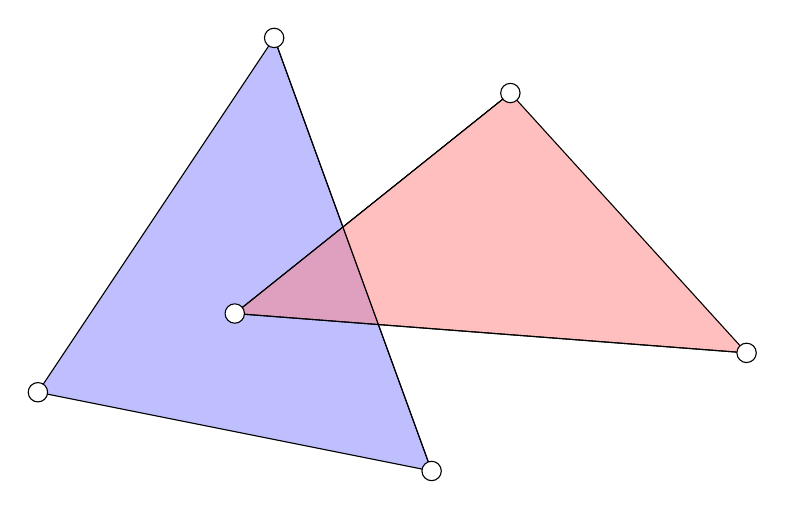
\begin{tikzpicture}[every node/.style={circle,draw=black, fill=white, inner sep=0pt,minimum size=7pt}]
      % Simplex 1
      \coordinate (A) at (0,0);
      \coordinate (B) at (3,4.5);
      \coordinate (C) at (5,-1);

      % Simplex 2
      \coordinate (D) at (2.5,1);
      \coordinate (E) at (6,3.8);
      \coordinate (F) at (9,.5);

      \draw[fill=blue!50!white, fill opacity=.5] (A) -- (B) -- (C) -- (A);
      \draw[fill=red!50!white, fill opacity=.5] (D) -- (E) -- (F) -- (D);

      \draw[name path=B--C] (B) -- (C);
      \draw[name path=D--E] (D) -- (E);
      \draw[name path=D--F] (D) -- (F);

      \path[name intersections={of=B--C and D--E, by=G}];
      \path[name intersections={of=B--C and D--F, by=H}];

      % nodes for simplex (1)
      \node (a) at (A) {};
      \node (b) at (B) {};
      \node (c) at (C) {};

      % nodes for simplex (2)
      \node (d) at (D) {};
      \node (e) at (E) {};
      \node (f) at (F) {};
    \end{tikzpicture}
    \caption{An unfortunate collision}
    \label{fig:non-simplicial-complex}
  \end{figure}
  Note that to fix this sorry situation, we can't just add two vertices at the
  points of intersections of the lines above (then the intersection of the
  resulting simplex with the two shone above would be non-trivial, but still not
  a face of the larger ones). We'd actually need something much more
  complicated.
  \begin{figure}[H]
    \centering
    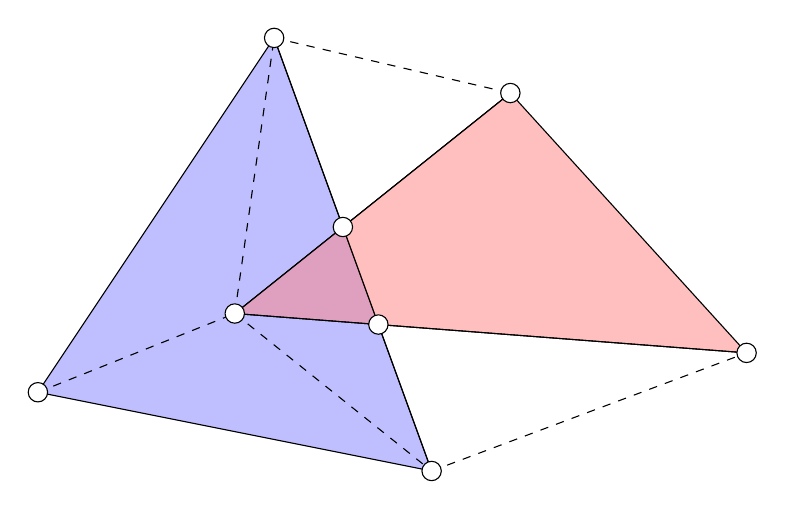
\begin{tikzpicture}[every node/.style={circle,draw=black, fill=white, inner sep=0pt,minimum size=7pt}]
      % Simplex 1
      \coordinate (A) at (0,0);
      \coordinate (B) at (3,4.5);
      \coordinate (C) at (5,-1);

      % Simplex 2
      \coordinate (D) at (2.5,1);
      \coordinate (E) at (6,3.8);
      \coordinate (F) at (9,.5);

      \draw[fill=blue!50!white, fill opacity=.5] (A) -- (B) -- (C) -- (A);
      \draw[fill=red!50!white, fill opacity=.5] (D) -- (E) -- (F) -- (D);

      \draw[name path=B--C] (B) -- (C);
      \draw[name path=D--E] (D) -- (E);
      \draw[name path=D--F] (D) -- (F);

      \path[name intersections={of=B--C and D--E, by=G}];
      \path[name intersections={of=B--C and D--F, by=H}];

      \draw[dashed] (B) -- (E);
      \draw[dashed] (C) -- (F);
      \draw[dashed] (A) -- (D);
      \draw[dashed] (D) -- (B);
      \draw[dashed] (D) -- (C);

      \node (g) at (G) {};
      \node (h) at (H) {};

      % nodes for simplex (1)
      \node (a) at (A) {};
      \node (b) at (B) {};
      \node (c) at (C) {};

      % nodes for simplex (2)
      \node (d) at (D) {};
      \node (e) at (E) {};
      \node (f) at (F) {};
    \end{tikzpicture}
    \caption{Constructing a resolution}
    \label{fig:constructing-a-resolution}
  \end{figure}
  \begin{figure}[H]
    \centering
    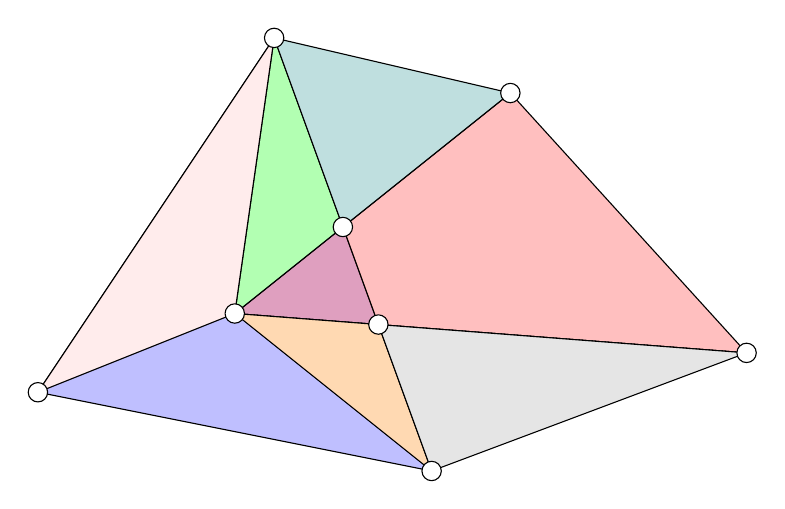
\begin{tikzpicture}[every node/.style={circle,draw=black, fill=white, inner sep=0pt,minimum size=7pt}]
      % Simplex 1
      \coordinate (A) at (0,0);
      \coordinate (B) at (3,4.5);
      \coordinate (C) at (5,-1);

      % Simplex 2
      \coordinate (D) at (2.5,1);
      \coordinate (E) at (6,3.8);
      \coordinate (F) at (9,.5);

      \draw[fill=blue!50!white, fill opacity=.5] (A) -- (B) -- (C) -- (A);
      \draw[fill=red!50!white, fill opacity=.5] (D) -- (E) -- (F) -- (D);

      \draw[name path=B--C] (B) -- (C);
      \draw[name path=D--E] (D) -- (E);
      \draw[name path=D--F] (D) -- (F);

      \path[name intersections={of=B--C and D--E, by=G}];
      \path[name intersections={of=B--C and D--F, by=H}];

      \draw[fill=green!30!white] (B) -- (G) -- (D) -- (B);
      \draw[fill=orange!30!white] (H) -- (C) -- (D) -- (H);
      \draw[fill=pink!30!white] (A) -- (B) -- (D) -- (A);
      \draw[fill=teal!25!white] (B) -- (E) -- (G) -- (B);
      \draw[fill=black!10!white] (H) -- (F) -- (C) -- (H);

      \node (g) at (G) {};
      \node (h) at (H) {};

      % nodes for simplex (1)
      \node (a) at (A) {};
      \node (b) at (B) {};
      \node (c) at (C) {};

      % nodes for simplex (2)
      \node (d) at (D) {};
      \node (e) at (E) {};
      \node (f) at (F) {};
    \end{tikzpicture}
    \caption{The completed resolution}
    \label{fig:completed-resolution}
  \end{figure}
\end{solution}
\begin{definition}[Underlying space]
  The \emph{underlying space} $\abs{K}$ of a simplicial complex $K$ is the set
  \[
    \abs{K} = \bigcup_{\sigma \in K} \sigma,
  \]
  the union of all simplices in $K$, with a topology consisting of sets whose
  intersection with each simplex $\sigma \in K$ is open in $\sigma$. For finite
  simplicial complexes, this topology is the topology inherited as a subspace of
  $\RR^n$.
\end{definition}
\begin{problem}[15.14]
  Let $K$ be the following simplicial complex:
  \[
    \text{(Omitted because it takes a long time to TeX out)}
  \]
  draw $K$ and its underlying space.
\end{problem}
\begin{solution}
  \begin{figure}[H]
    \centering
    \begin{minipage}{.49\linewidth}
      \centering
      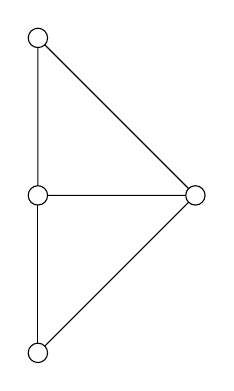
\begin{tikzpicture}[scale=2, every node/.style={circle,draw=black, fill=white, inner sep=0pt,minimum size=7pt}]

        \coordinate (A) at (0,0);
        \coordinate (B) at (0,1);
        \coordinate (C) at (1,0);
        \coordinate (D) at (0,-1);

        \draw (A) -- (B) -- (C) -- (A);
        \draw (A) -- (D);
        \draw (D) -- (C);

        \node (a) at (A) {};
        \node (b) at (B) {};
        \node (c) at (C) {};
        \node (d) at (D) {};

      \end{tikzpicture}
    \end{minipage}
    \begin{minipage}{.49\linewidth}
      \centering
      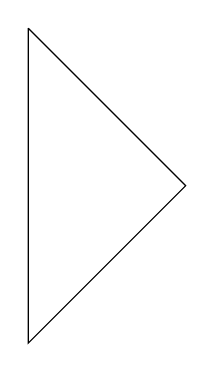
\begin{tikzpicture}[scale=2, every node/.style={circle,draw=black, fill=white, inner sep=0pt,minimum size=7pt}]

        \coordinate (B) at (0,1);
        \coordinate (C) at (1,0);
        \coordinate (D) at (0,-1);

        \draw (B) -- (C) -- (D) -- (B);
      \end{tikzpicture}
    \end{minipage}
    \caption{$K$ (left) and its underlying space (right).}
  \end{figure}
\end{solution}
\begin{definition}[Triangulable]
  A topological space $X$ is said to be \emph{triangulable} if it is
  homeomorphic to the underlying space of a simplicial complex $K$. In that
  case, we say $K$ is a \emph{triangulation} of $X$.
\end{definition}
\begin{problem}[15.15]
  Show that the space shown in Figure 15.2 (not included here) is triangulable
  by exhibiting a simplicial complex whose underlying space it is homeomorphic
  to.
\end{problem}
\begin{solution}
  \begin{figure}[H]
    \centering
    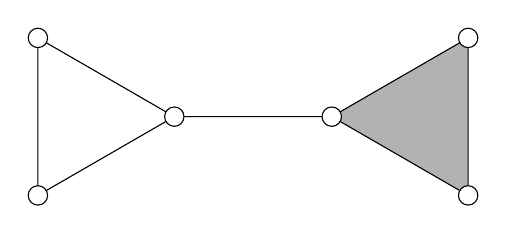
\begin{tikzpicture}[scale=2, every node/.style={circle,draw=black, fill=white, inner sep=0pt,minimum size=7pt}]

      \coordinate (A) at (0,0);
      \coordinate (B) at (-.866,.5);
      \coordinate (C) at (-.866,-.5);
      \coordinate (D) at (1,0);
      \coordinate (E) at (1.866,.5);
      \coordinate (F) at (1.866,-.5);

      \draw (A) -- (B) -- (C) -- (A) -- (D);
      \draw[fill=black!30!white] (D) -- (E) -- (F) -- (D);

      \node (a) at (A) {};
      \node (b) at (B) {};
      \node (c) at (C) {};
      \node (d) at (D) {};
      \node (e) at (E) {};
      \node (f) at (F) {};

    \end{tikzpicture}
    \caption{Such a simplicial complex. Note, the left triangle is unfilled.}
  \end{figure}
\end{solution}
\begin{problem}[15.6]
  For each $n \in \NN$, $\sS^n$ is triangulable.
\end{problem}
\begin{proof}
  We proceed by induction.

  \begin{induction}
    \item Note that $S^0$ is trivially triangulable by taking $K =
      \set{\set{v_0}, \set{v_2}}$.
    \item Suppose that for $k \in \NN \cup \set{0}$, $\sS^k$ is triangulable by
      a simplicial complex $K$.
    \item Take $v_{k+1} \in \RR^{k+1}$ such that $v_{k+1} \in
      (\vspan{K})^\perp$. Then
  \end{induction}
  {\color{red} This proof is unfinished. Hey, future Forest --- you should
    return to this later!}
\end{proof}
\section{Simplicial Maps and PL Homeomorphisms}
We now define structure-preserving maps bewteen simplicial concepts.
\begin{definition}[Simplicial map]
  Let $X,Y$ be topological spaces. A function $f : X \to Y$ is called a
  \emph{simplicial map} iff there exist simplicial complexes $K$ and $L$ such
  that $\abs{K} = X$, $\abs{L} = Y$, and $f$ maps each simplex of $K$ linearly
  onto a (possibly lower-dimensional) simplex in $L$.
\end{definition}
\begin{definition}[Simplicially homeomorphic]
  A simplicial map $f$ is a simplicial homomorphism iff it's a bijection; in
  that case, the two complexes are \emph{simplicially homeomorphic}
\end{definition}
\begin{problem}[15.17]
  A simplicial map from $K$ to $L$ is determined by the images of the vertices
  of $K$.
\end{problem}
\begin{solution}
  Apply linearity and show the analog of images of liner combinations being
  uniquely determined by the action on the basis.
\end{solution}
\begin{problem}[15.18]
  A composition of simplicial maps is a simplicial map.
\end{problem}
\begin{solution}
  Simply plug in arbitrary points and verify the properties hold.
\end{solution}
\begin{definition}[Subdivision]
  Let $K$ be a simplicial complex. Then a simplicial complex $K'$ is a
  \emph{subdivision} of $K$ iff each simplex of $K'$ is a subset of a simplex of
  $K$ and each simplex of $K$ is the union of finitely many simplices of $K'$.
\end{definition}
\begin{definition}[Piecewise linear]
  If $K$ and $L$ are complexes, a continuous map $f : \abs{K} \to \abs{L}$ is
  called \emph{piecewise linear} or \emph{PL} if and only if there are
  subdivisions $K'$ of $K$ and $L'$ of $L$ such that $f$ is a simplicial map
  from $K'$ to $L'$. If there exist subdivisions such that $f$ is a simplicial
  homomorphism, then $f$ is a \emph{PL homeomorphism} and the spaces are
  \emph{PL homeomorphic.}
\end{definition}
\begin{problem}[15.21]
  A composition of PL maps is PL. A PL homeomorphism is an equivalence relation.
\end{problem}
\begin{solution}
  Let $K,L,M$ be complexes, and let $g : \abs{K} \to \abs{L}$, $f : \abs{L} \to
  \abs{M}$ be continuous PL maps. WTS $h = f \circ g$ is a PL map.

  Let $K', L', M'$ be the corresponding subdivisions of $K,L,$ and $M$,
  respectively. Then $g$ is a simplicial map from $K'$ to $L'$, and $f$ is a
  simplicial map from $L'$ to $M'$. Then $\forall \sigma \in K'$, $g(\sigma) \in
  L'$, whence $f(g(\sigma)) \in M'$. It follows that $h = g \circ f$ is a
  simplicial map from $K'$ to $M'$.

  We give a sketch of the proof that PL homeomorphism is an equivalence
  relation. To verify reflexivity, take the identity map. Symmetry follows by
  inverting the simplicial homeomorphism. Transitivity follows by the above.
  Thus, the claim holds.
\end{solution}
% \begin{problem}[15.22]
%   PL homeomorphic complexes are homeomorphic as topological spaces.
% \end{problem}
% \begin{solution}
% \end{solution}
\section{Simplicial Approximation}
\begin{problem}[15.23]
  Let $K$ be a complex consisting of the boundary of a triangle (three vertices
  and three edges) and $L$ be an isomorphic complex. Both $\abs{K}$ and
  $\abs{L}$ are topologically circles. There is a continuous map that takes the
  circle $\abs{K}$ and winds it twice around the circle $\abs{L}$; however, show
  that there is no simplicial map from $K$ to $L$ that winds the circle
  $\abs{K}$ twice around the circle $\abs{L}$.
\end{problem}
\begin{solution}
  We offer a brief sketch. Basically, this would require each 1-simplex to map
  to two 1-simplices. Contradiction.
\end{solution}
\begin{definition}[Barycenter]
  The \emph{barycenter} of a $k$-simplex $\simp{k}$ in $\RR^n$ is the point
  $\frac{1}{k+1} \pn{v_0 + \cdots + v_k}$.
\end{definition}
\begin{definition}[First barycentric subdivision ($\sd \sigma$)]
  Let $\sigma$ be an $n$-simplex. The \emph{first barycentric subdivision of
    $\sigma$}, denoted $\sd \sigma$, is the complex of all simplices of the form
  $\simp[b]{k}$, where $b_i$ is the barycenter of a face $\sigma^i$ of $\sigma$
  from a chain of faces of $\sigma$,
  \[
    \sigma^0 \subset \sigma^1 \subset \cdots \subset \sigma^k
  \]
  of increasing (not necessarily consecutive) dimensions. The maximal simplices,
  that is, the $n$-simplices of $\sd \sigma$ each arise from a maximal sequence
  of faces, that is, from faces of consecutive dimensions starting with a vertex
  of $\sigma$. Thus an $n$-simplex of $\sd \sigma$ corresponds exactly to a
  permutation of the vertices of $\sigma$.
\end{definition}
\begin{definition}[$\sd K$]
  Let $K$ be a simplicial complex. The \emph{first barycentric subdivision} of
  $K$, denoted $\sd K$, is the complex consisting of all the simplices in the
  barycentric subdivision of each simplex of $K$.
\end{definition}
\begin{definition}[$m$-th barycentric subdivision]
  The \emph{second barycentric subdivision}, denoted $\sd^2 K$, is the first
  barycentric subdivision of $\sd K$. Proceeding in this way, the \emph{$m$-th
    barycentric subdivision} is denoted $\sd^m K$.
\end{definition}
Some diagrams:
\begin{figure}[H]
  \centering
  \begin{subfigure}{.45\linewidth}
    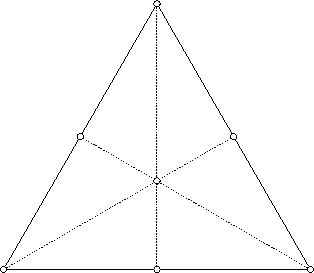
\includegraphics[width=\linewidth]{figures/barycentric-1.pdf}
  \end{subfigure}
  \hspace{1cm}
  \begin{subfigure}{.45\linewidth}
    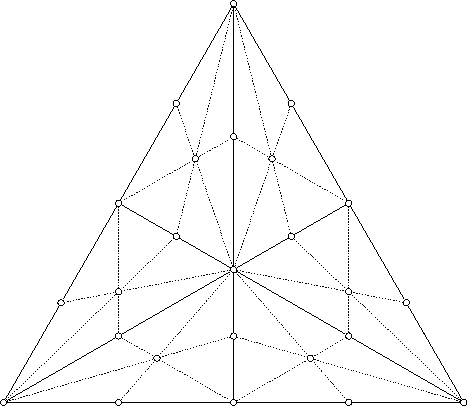
\includegraphics[width=\linewidth]{figures/barycentric-2.pdf}
  \end{subfigure}\\[2cm]
  \begin{subfigure}{.45\linewidth}
    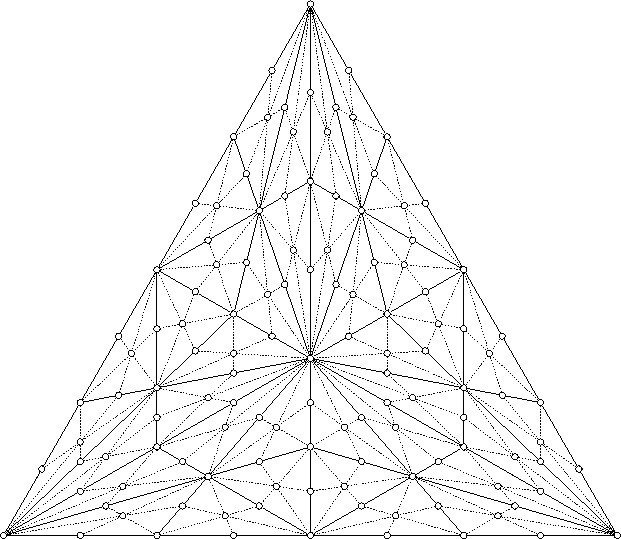
\includegraphics[width=\linewidth]{figures/barycentric-3.pdf}
  \end{subfigure}
  \hspace{1cm}
  \begin{subfigure}{.45\linewidth}
    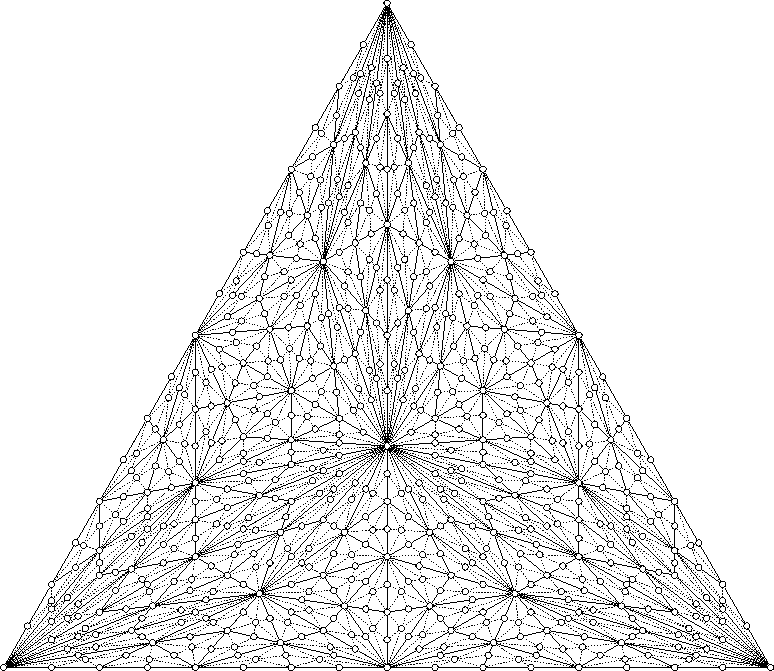
\includegraphics[width=\linewidth]{figures/barycentric-4.pdf}
  \end{subfigure}
  \caption{The first 4 barycentric subdivisions}
  \label{fig:subdivs}
\end{figure}
\begin{problem}[15.24]
  How many $n$-simplices are there in the first barycentric subdivision of an
  $n$-simplex?
\end{problem}
\begin{solution}
  A simple induction shows there are $6^n$ $n$-simplices.
\end{solution}
\begin{problem}[15.25]
  Convince yourself that the barycentric subdivision of a complex $K$ is, in
  fact, a subdivision of $K$.
\end{problem}
\begin{solution}
  I'm convinced.
\end{solution}
\begin{problem}[15.26]
  Let $K$ be a finite simplicial complex and let $a_n$ be the maximum among the
  diameters of simplices in $\sd^n K$. Then
  \[
    \lim_{n\to\infty} a_n = 0.
  \]
\end{problem}
\begin{solution}
  First, we calculate the diameter of an $n$-simplex.
  \begin{leftbar}
    \begin{lemma}
      Let $\sigma_n$ be an $n$-simplex. Then the diameter of $\sigma_n$
      \[
        D = \sup_{\mathclap{\Xx,\, \Yy \in \sigma_n}} \norm{\Xx - \Yy}_2
      \]
      is given by the maximum distance between vertices in the simplex:
      \[
        D = \sup_{\mathclap{\Vv_i, \Vv_j}} \norm{\Vv_i - \Vv_j}_2
      \]
    \end{lemma}

    \emph{Proof of Lemma:} Let $\Xx, \Yy \in \sigma_n$ be arbitrary. It will
    suffice to show that $\Yy$ is not a vertex in $\sigma_n$, then there exists
    a vertex $\Vv \in \sigma_n$ such that $\norm{\Xx - \Yy}_2 < \norm{\Xx -
      \Vv}_2$.

    Write $\Yy$ as convex combinations by
    \begin{align*}
      \Yy &= \sum_{i=0}^n \mu_i \Vv_i.
    \end{align*}
    and observe that since $\sum_{i=0}^n \mu_i = 1$, we have
    \[
      \Xx = \sum_{i=0}^n \mu_i \Xx = \Xx.
    \]
    Then
    \begin{align*}
      \norm{\Xx - \Yy}_2
      &= \norm{\sum_{i=0}^n \Xx - \mu_i\Vv_i}_2 \\
      &= \norm{\sum_{i=0}^n \mu_i(\Xx - \Vv_i)}_2 \\
      &\leq \sum_{i=0}^n \mu_i \norm{\Xx - \Vv_i}_2 \\
      &\leq \sum_{i=0}^n \mu_i \sup_{\Vv_i} \norm{\Xx - \Vv_i}_2 \\
      &= \sup_{\Vv_i} \norm{\Xx - \Vv_i}_2.
    \end{align*}
    Hence, we see for arbitrary $\Yy$, $\norm{\Xx - \Yy}_2 \leq \sup_{\Vv_i}
    \norm{\Xx - \Vv_i}_2$. Now, apply the same result to $\Xx' = \argmax_{\Vv_i}
    \norm{\Xx - \Vv_i}_2$ and $\Yy' = \Xx$ to obtain
    \[
      \norm{\Xx - \Yy}_2 \leq \sup_{\Vv_i} \norm{\Xx - \Vv_i}_2 \leq
      \sup_{\Vv_j}\pn{ \sup_{\Vv_i} \norm{\Vv_j - \Vv_i}} = \sup_{\Vv_i, \Vv_j}
      \norm{\Vv_j - \Vv_i}_2
    \]
    as desired.
  \end{leftbar}
  By the lemma, $a_n$ is given by the maximal side length of a 2-simplex in
  $\sd^n K$. Hence
  \[
    0 \leq a_n \leq \frac{1}{2^n} \frac{2}{\sqrt{3}} \quad \text{\color{red}
      This bound is incorrect. How can I fix it?}
  \]
  and so by the squeeze theorem,
  \[
    \lim_{n\to\infty} a_n = 0
  \]
  as desired.
\end{solution}
\begin{definition}[Minimal face]
  Let $K$ be a simplicial complex. The \emph{minimal face} of $x \in \abs{K}$ is
  the simplex of $K$ of smallest dimension that contains $x$.
\end{definition}
\begin{definition}[Star of vertex]
  The \emph{star of a vertex} $v$ in $K$, denoted $\St(v)$, is the set of all
  points whose minimal face contains $v$.
\end{definition}
\begin{remark}
  The definition of the star of a vertex is basically the interior of the union
  of all simplices containing $v$.
\end{remark}
\begin{problem}[15.27]
  The star of a vertex $v$ in a complex $K$ is an open set of $\abs{K}$, and the
  collection of all vertex stars covers $\abs{K}$.
\end{problem}
\begin{solution}
  Let $v \in K$ be a vertex. Let $x \in \St(v)$ be arbitrary. WTS $\exists
  \varepsilon > 0 \st B_{\epsilon}(x) \subset \St(v)$. We have the following
  cases:
  \begin{enumerate}[label=(\arabic*)]
    \item Suppose $x = v$. Then taking $\epsilon = \frac{1}{2} \inf_{\Vv_i}
      \abs{v - \Vv_i}_2$ we get the desired result.
    \item Suppose $x \neq v$. Then taking $v = v_0$, write $x$ in the
      barycentric coordinates
      \[
        x = \lambda_0 v + \lambda_1 v_1 + \cdots + \lambda_n v_n.
      \]
      Since $x \in \St(v)$, $\lambda_0 \neq 0$.
  \end{enumerate}
\end{solution}
\begin{problem}[15.28]
  If the simplex $\sigma = \simp{k}$ in $K$ is the minimal face of a point $x
  \in \abs{K}$, then
  \[
    x \in \bigcap_{i=0}^n \St(v_0)
  \]
\end{problem}
\begin{solution}

\end{solution}
%%% Local Variables:
%%% TeX-master: "../main"
%%% End:
\chapter[$\zmod{2}$ Homology]{Simplicial $\ZZ_2$-Homology: Physical Algebra}
\section{Intro}
This chapter, we'll talk about \emph{homology}, which captures holes in a much
more satisfying way than higher homotopy groups do.
\begin{adjustwidth}{1.5em}{}
  \begin{remark}
    Although not exactly accurate, a good way to start to understand homology for
    a space $X$ is to view an $n$-manifold in $X$ that is not the boundary of an
    $(n+1)$-manifold-with-boundary as capturing some geometry of $X$ while an
    $n$-manifold that is the boundary of an $(n+1)$-dimensional
    manifold-with-boundary is not detecting any hole or structure.
  \end{remark}
\end{adjustwidth}
\section{Chains, Cycles, Boundaries, and the Homology Groups}
\begin{definition}
  An \emph{$n$-chain} of $K$ is a finite formal sum
  \[
    \sum_{i=1}^k \sigma_i
  \]
  of distinct $n$-simplices in $K$. Note that the dimensions of the simplices
  must be the same. So \emph{chain} will mean $n$-chain whenever the dimension
  is either unimportant or understood.
\end{definition}
\begin{definition}
  The \emph{$n$-chain group of $K$} (with coefficients in $\zmod{2}$), denoted
  $\mathsf{C}_n(K)$, is the collection of $n$-chains in $K$ under formal
  addition modulo 2. If there are no $n$-simplices in $K$, the $n$-chain group
  of $K$ is defined to be trivial (containing the ``empty'' chain).
\end{definition}
\begin{problem}[16.1]
  Check that $\msf C_n(K)$ is an abelian group.
\end{problem}
\begin{solution}
  \begin{enumerate}[label=(\arabic*)]
  \item $\epsilon = \sum_{i \in \varnothing} \sigma_i$.
  \item Associativity inherited from $\cup$.
  \item Closure inherited from $\cup$ over the domain given.
  \item Existence of inverses --- since we're taking formal linear
    combinations over $\zmod{2}$, then every element is its own inverse.
  \end{enumerate}
  Finally, to see that $\msf C_n(K)$ is abelian, observe that $+$ in $\msf
  C_n(K)$ inherits commutativity from $\cup$.
\end{solution}
\begin{definition}
  The \emph{$\zmod{2}$-boundary of an $n$-simplex $\sigma = \simp{n}$} is
  defined by
  \[
    \partial \sigma = \sum_{i=0}^n \simpdel{i}{n}
  \]
  the formal sum of the $(n-1)$-faces of $\sigma$.

  For a 0-simplex, the $\zmod{2}$ boundary is defined to be $0 \in \msf
  C_{-1}(K)$.
\end{definition}
\begin{definition}
  The \emph{$\zmod{2}$ boundary of an $n$-chain} is the sum of the boundaries of
  the simplices. That is, $\partial_n : \msf C_n(K) \to \msf C_{n-1}(K)$ is
  given by
  \[
    \partial\pn{\sum_{i=1}^k \sigma_i} = \sum_{i=1}^k \partial(\sigma_i)
  \]
\end{definition}
\begin{problem}[16.2]
  Verify that $\partial$ is a homomorphism, and use the definition to compute
  the $\zmod{2}$ boundary of $\sigma_1 + \sigma_2$ in Figure 16.1
\end{problem}
\begin{solution}
  We want to show $\partial$ is a homomorphism.
  \begin{enumerate}
  \item Let $\epsilon_n \in \msf C_n(K)$ be identity. We want to show
    $\partial(\epsilon_n) = \epsilon_{n-1}$. Taking the empty sum to be
    identity, we see
    \begin{align*}
      \partial(\epsilon_n)
      &=
        \partial\pn{\sum_{i\in \varnothing} \sigma_i} \\
      &= \sum_{i\in\varnothing} \partial\pn{\sigma_i} \\
      &= \epsilon_{n-1}
    \end{align*}
    as desired.
  \item That $\partial$ respects addition is definitional.
  \end{enumerate}
  We have $\partial(\sigma_1 + \sigma_2) = e_1 + e_2 + e_4 + e_5$.
\end{solution}
\begin{definition}
  An \emph{$n$-cycle} is an $n$-chain of $K$ whose boundary is zero. The set of
  all $n$-cycles on $K$ is denoted $\msf Z_n(K)$. An \emph{$n$-boundary} is an
  $n$-chain that is the boundary of an $(n+1)$-chain of $K$. The set of all
  $n$-boundaries is denoted $\msf B_n(K)$.
\end{definition}
% \begin{problem}[16.3]

% \end{problem}
\begin{problem}[16.4]
  Both $\msf Z_n(K)$ and $\msf B_n(K)$ are subgroups of $\msf C_n(K)$. Moreover,
  \[
    \partial \circ \partial = 0.
  \]
  In other words, $\partial_n \circ \partial_{n+1} = 0$ for each index $n \geq
  0$. Hence, $\msf B_n(K) \subset \msf Z_n(K)$.
\end{problem}
\begin{solution}
  Let $\sigma_1, \sigma_2 \in \msf Z_n(K)$. Then by linearity of $\partial_n$,
  we have
  \begin{align*}
    \partial_n(\sigma_1 + \sigma_2)
    &= \partial_n(\sigma_1) + \partial_n(\sigma_2) \\
    &= 0
  \end{align*}
  and hence $\msf Z_n(K) < \msf C_n(K)$.

  Now, let $\sigma_1, \sigma_2 \in \msf B_n(K)$. Then $\exists \tau_1, \tau_2
  \in \msf Z_{n+1}(K)$ such that $\partial_{n+1}(\tau_1) = \sigma_1,
  \partial_{n+1}(\tau_2) = \sigma_{2}$. Since $\msf Z_{n+1}(K) < \msf
  C_{n+1}(K)$, then $\tau_1 + \tau_2 \in \msf Z_{n+1}(K)$. Now, by linearity of
  $\partial$, we have
  \begin{align*}
    \partial_{n+1}(\tau_1 + \tau_2)
    &= \partial_{n+1}(\tau_1) + \partial_{n+1}(\tau_2) \\
    &= \sigma_1 + \sigma_2
  \end{align*}
  hence $\msf B_n(K)$ is a subset closed under the operation, so we have $\msf
  B_n(K) < \msf C_n(K)$.

  It remains to show $\partial_n \circ \partial_{n+1} = 0$. Let $\sigma \in \msf
  C_{n+1}(K)$. Then
  \begin{align*}
    \partial_{n+1}(\sigma)
    &= \partial_{n+1}\pn{\sum_{i \in I} \simp[v^{(i)}]{n+1}} \\
    &= \sum_{i\in I} \partial_{n+1}\pn{\simp[v^{(i)}]{n+1}} \\
    &= \sum_{i\in I} \sum_{j \in [n+1]} \simpdel[v^{(i)}]{j}{n+1}
  \end{align*}
  and so
  \begin{align*}
    \partial_n \pn{\partial_{n+1}(\sigma)}
    &= \sum_{i\in I} \sum_{j \in [n+1]} \partial_{n}\pn{\simpdel[v^{(i)}]{j}{n+1}} \\
    &= \sum_{i\in I} \sum_{j \in [n+1]} \sum_{\substack{k \in [n+1] \\ k \neq j}} \set{v_0^{(i)} \cdots \widehat{v_k^{(i)}} \cdots \widehat{v_j^{(i)}}\cdots v^{(i)}_{n+1}}
  \end{align*}
  hence all the terms cancel, and we're left with $\mb 0$. So $\partial_n \circ
  \partial_{n+1} = 0$, as desired.

  Since every $\sigma \in \msf B_n(K)$ is of the form $\partial_{n+1}(\tau)$
  where $\tau \in \msf C_{n+1}(K)$, it follows that $\partial_n\fim[\msf
  B_n(K)] = (\partial_n \circ \partial_{n+1}) (\msf C_{n+1}(K)) = 0$. Thus $\msf
  B_n(K) < \msf Z_n(K)$.
\end{solution}
\begin{definition}
  Two $n$-cycles $\alpha$ and $\beta$ in $K$ are \emph{equivalent} or
  \emph{homologous} iff $\alpha-\beta = \partial(\gamma)$ for some $(n+1)$-chain
  $\gamma$. In other words, $\alpha$ and $\beta$ are homologous iff they differ
  by an element of the subgroup $\msf B_n(K)$, denoted by
  \[
    \alpha \sim_{\zmod{2}} \beta.
  \]
  The equivalence class of $\alpha$ is denoted by enclosing it in brackets
  thusly: $[\alpha]$. For $\zmod{2}$ $n$-chains, observe that $\alpha - \beta =
  \alpha + \beta$. So we see that two $n$-cycles are equivalent if together they
  bound an $(n+1)$-chain.
\end{definition}
\begin{definition}
  The \emph{$n$\textsuperscript{th}-homology group} (with coefficients in
  $\zmod{2}$) of a finite simplicial complex $K$, denoted $\msf H_n(K)$, is the
  additive group whose elements are equivalence classes of cycles under the
  $\zmod{2}$-equivalence defined above, with $\bk{\alpha} + \bk{\beta} =
  \bk{\alpha +\beta}$. I.e.,
  \[
    \msf H_n(K) = \msf Z_n(K)/\msf B_n(K)
  \]
\end{definition}
\begin{problem}[F1]
  Consider the simplicial complex given below in Figure \cref{fig:F1}. Then for
  $n = 0, 1, 2$,
  \begin{enumerate}
  \item describe elements of $\msf C_n(K)$,
  \item compute $\msf Z_n(K)$,
  \item compute $\msf B_n(K)$, and
  \item compute $\msf H_n(K)$.
  \end{enumerate}
\end{problem}
\begin{figure}[H]
  \centering
  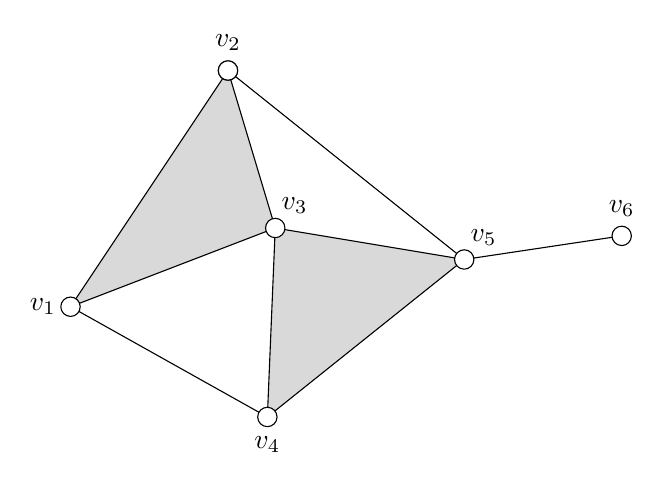
\begin{tikzpicture}[
    every node/.style={
      circle,
      draw=black,
      fill=white,
      inner sep=0pt,
      minimum size=7pt
    }
    ]

    \coordinate (v1) at (0,0);
    \coordinate (v2) at (2,3);
    \coordinate (v3) at (2.6,1);
    \coordinate (v4) at (2.5,-1.4);
    \coordinate (v5) at (5,.6);
    \coordinate (v6) at (7,.9);

    \draw[fill=gray!30!white] (v1) -- (v2) -- (v3) -- (v1) -- cycle;
    \draw[fill=gray!30!white] (v3) -- (v4) -- (v5) -- (v3) -- cycle;

    \draw (v1) -- (v4);
    \draw (v2) -- (v5);
    \draw (v5) -- (v6);

    \node (wv1) at (v1) {};
    \node (wv2) at (v2) {};
    \node (vv2) at (v2) {};
    \node (vv3) at (v3) {};
    \node (vv4) at (v4) {};
    \node (vv5) at (v5) {};
    \node (vv6) at (v6) {};

    \node[draw=none, xshift=-1em] (wv1) at (v1) {$v_1$};
    \node[draw=none, yshift=1em] (wv2) at (v2) {$v_2$};
    \node[draw=none, xshift=.7em, yshift=.8em] (wv3) at (v3) {$v_3$};
    \node[draw=none, yshift=-1em] (wv4) at (v4) {$v_4$};
    \node[draw=none, xshift=.7em, yshift=.8em] (wv5) at (v5) {$v_5$};
    \node[draw=none, yshift=1em] (wv6) at (v6) {$v_6$};
  \end{tikzpicture}
  \caption{Simplicial complex $K$}
  \label{fig:F1}
\end{figure}
\begin{solution}
  First, we redraw the simplicial complex as follows:
  \begin{figure}[H]
    \centering
    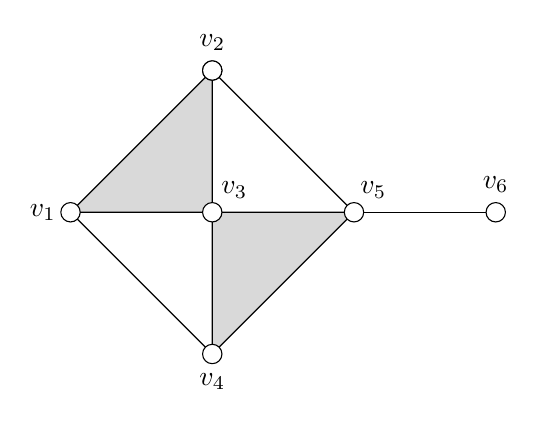
\begin{tikzpicture}[
      scale = .6,
      every node/.style={
        circle,
        draw=black,
        fill=white,
        inner sep=0pt,
        minimum size=7pt
      }
      ]

      \coordinate (v1) at (-3,0);
      \coordinate (v2) at (0,3);
      \coordinate (v3) at (0,0);
      \coordinate (v4) at (0,-3);
      \coordinate (v5) at (3,0);
      \coordinate (v6) at (6,0);

      \draw[fill=gray!30!white] (v1) -- (v2) -- (v3) -- (v1) -- cycle;
      \draw[fill=gray!30!white] (v3) -- (v4) -- (v5) -- (v3) -- cycle;

      \draw (v1) -- (v4);
      \draw (v2) -- (v5);
      \draw (v5) -- (v6);

      \node (wv1) at (v1) {};
      \node (wv2) at (v2) {};
      \node (vv2) at (v2) {};
      \node (vv3) at (v3) {};
      \node (vv4) at (v4) {};
      \node (vv5) at (v5) {};
      \node (vv6) at (v6) {};

      \node[draw=none, xshift=-1em] (wv1) at (v1) {$v_1$};
      \node[draw=none, yshift=1em] (wv2) at (v2) {$v_2$};
      \node[draw=none, xshift=.8em, yshift=.8em] (wv3) at (v3) {$v_3$};
      \node[draw=none, yshift=-1em] (wv4) at (v4) {$v_4$};
      \node[draw=none, xshift=.7em, yshift=.8em] (wv5) at (v5) {$v_5$};
      \node[draw=none, yshift=1em] (wv6) at (v6) {$v_6$};
    \end{tikzpicture}
    \caption{Simplicial complex $K$, straightened out}
  \end{figure}
  For the purposes of this problem, take angled brackets indicate span. We have
  \begin{enumerate}[label=(\roman*)]
  \item We calculate the $k=0$ case.
    \begin{enumerate}
    \item Elements of $\msf C_0(K)$ are formal linear combinations over the
      set $\set{v_1, v_2, \ldots, v_6}$. Then
      \[
        \msf C_0(K) = \ip[Big]{v_1, v_2, v_3, v_4, v_5, v_6}
      \]
      that is, collections of points in $\msf C_0(K)$.
    \item Let $\sigma_1, \ldots, \sigma_k \in \msf C_0(K).$ Then by definition,
      \begin{align*}
        \partial\pn{\sum_{i=1}^k \sigma_i}
        &= \sum_{i=1}^k \partial(\sigma_i)\\
        &= \sum_{i=1}^k 0 \\
        &= 0
      \end{align*}
      hence $\msf Z_n(K) = \msf C_n(K)$.
    \item A $\sigma \in \msf C_0(K)$ is an $n$-boundary if $\exists \tau \in
      \msf C_{1}(K)$ with $\partial(\tau) = \sigma$. Note, for any
      $1$-dimensional face $\set{v_iv_j} \in K$,
      \begin{align*}
        \partial(\set{v_iv_j})
        &= \set{v_i \widehat{v_j}} + \set{\widehat{v_i}v_j} \\
        &= \set{v_i} + \set{v_j} \\
        &= \delta_{ij}.
      \end{align*}
      Hence, any edge formed of a pair of two distinct vertices yields a
      nonempty boundary. We first count all edges:
      \begin{figure}[H]
        \centering
        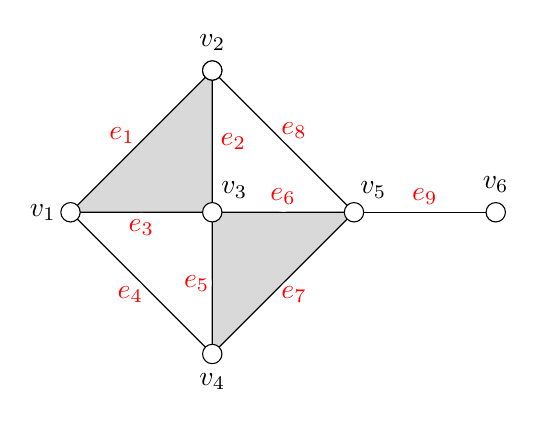
\begin{tikzpicture}[
          scale = .6,
          every node/.style={
            circle,
            draw=black,
            fill=white,
            inner sep=0pt,
            minimum size=7pt
          }
          ]

          \coordinate (v1) at (-3,0);
          \coordinate (v2) at (0,3);
          \coordinate (v3) at (0,0);
          \coordinate (v4) at (0,-3);
          \coordinate (v5) at (3,0);
          \coordinate (v6) at (6,0);

          \draw[fill=gray!30!white] (v1) -- (v2)
          % draw and label the edge between v1 and v2
          node[draw=none, midway, above left, xshift=-.3em, yshift=-.2em]
          {\color{red} $e_1$} -- (v3)
          % draw the edge between v2 and v3, and label it as well
          node[draw=none, midway, right, xshift=.2em] {\color{red} $e_2$}
          -- (v1)
          % draw the edge between v3 and v1, and label it as well
          node[draw=none, midway, below] {\color{red}$e_3$} -- cycle;

          \draw (v1) -- (v4) node[draw=none, midway, below left] {\color{red} $e_4$};

          \draw[fill=gray!30!white] (v3) -- (v4)
          % edge between v3 and and v4
          node[draw=none, midway, left] {\color{red} $e_5$} -- (v5)
          % edge
          node[draw=none, midway, below right] {\color{red}$e_7$} -- (v3)
          %
          node[draw=none, midway, above] {\color{red} $e_6$} -- cycle;


          \draw (v2) -- (v5) node[draw=none, midway, above right] {\color{red} $e_8$};
          \draw (v5) -- (v6) node[draw=none, midway, above] {\color{red} $e_9$};

          \node (wv1) at (v1) {};
          \node (wv2) at (v2) {};
          \node (vv2) at (v2) {};
          \node (vv3) at (v3) {};
          \node (vv4) at (v4) {};
          \node (vv5) at (v5) {};
          \node (vv6) at (v6) {};

          \node[draw=none, xshift=-1em] (wv1) at (v1) {$v_1$};
          \node[draw=none, yshift=1em] (wv2) at (v2) {$v_2$};
          \node[draw=none, xshift=.8em, yshift=.8em] (wv3) at (v3) {$v_3$};
          \node[draw=none, yshift=-1em] (wv4) at (v4) {$v_4$};
          \node[draw=none, xshift=.7em, yshift=.8em] (wv5) at (v5) {$v_5$};
          \node[draw=none, yshift=1em] (wv6) at (v6) {$v_6$};
        \end{tikzpicture}
        \caption{Simplicial complex $K$ with simple edges}
      \end{figure}
      Since $\msf B_0(K)$ is a subgroup of $\msf C_0(K)$, by closure under
      $+$, we see that any $v_i+v_j$ in $K$ such that there exists a path
      from $v_i$ to $v_j$ (when $K$ is considered a graph) is an element of
      $\msf B_0(K)$. In fact, we can say more:

      \textbf{Claim:} Since $K$ is connected as a graph, any even collection
      of vertices is in $\msf B_n(K)$.

      \textbf{Proof of Claim:} Suppose we have $\sigma = \set{v_{i_1}} +
      \set{v_{i_2}} + \cdots + \set{v_{i_{2k}}}$, where $k \in \NN$. Then
      for each $j = 1, \ldots, k$, let $\tau_j$ be a sum of edges representing
      a path from $v_{i_j}$ to $v_{i_{j+1}}$. For example, if $v_{i_j} =
      v_6$ and $v_{i_{j+1}} = v_2$, we could take the following approaches:
      \begin{figure}[H]
        \centering
        \begin{subfigure}{.49\linewidth}
          \centering
          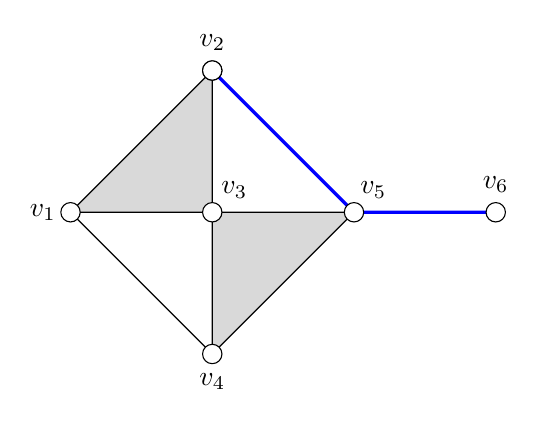
\begin{tikzpicture}[
            scale = .6,
            every node/.style={
              circle,
              draw=black,
              fill=white,
              inner sep=0pt,
              minimum size=7pt
            }
            ]

            \coordinate (v1) at (-3,0);
            \coordinate (v2) at (0,3);
            \coordinate (v3) at (0,0);
            \coordinate (v4) at (0,-3);
            \coordinate (v5) at (3,0);
            \coordinate (v6) at (6,0);

            \draw[fill=gray!30!white] (v1) -- (v2) -- (v3) -- (v1) -- cycle;
            \draw[fill=gray!30!white] (v3) -- (v4) -- (v5) -- (v3) -- cycle;

            \draw (v1) -- (v4);
            \draw (v2) -- (v5);
            \draw (v5) -- (v6);

            \draw[draw=blue, very thick] (v6) -- (v5) -- (v2);

            \node (wv1) at (v1) {};
            \node (wv2) at (v2) {};
            \node (vv2) at (v2) {};
            \node (vv3) at (v3) {};
            \node (vv4) at (v4) {};
            \node (vv5) at (v5) {};
            \node (vv6) at (v6) {};

            \node[draw=none, xshift=-1em] (wv1) at (v1) {$v_1$};
            \node[draw=none, yshift=1em] (wv2) at (v2) {$v_2$};
            \node[draw=none, xshift=.8em, yshift=.8em] (wv3) at (v3) {$v_3$};
            \node[draw=none, yshift=-1em] (wv4) at (v4) {$v_4$};
            \node[draw=none, xshift=.7em, yshift=.8em] (wv5) at (v5) {$v_5$};
            \node[draw=none, yshift=1em] (wv6) at (v6) {$v_6$};
          \end{tikzpicture}
        \end{subfigure}
        \begin{subfigure}{.49\linewidth}
          \centering
          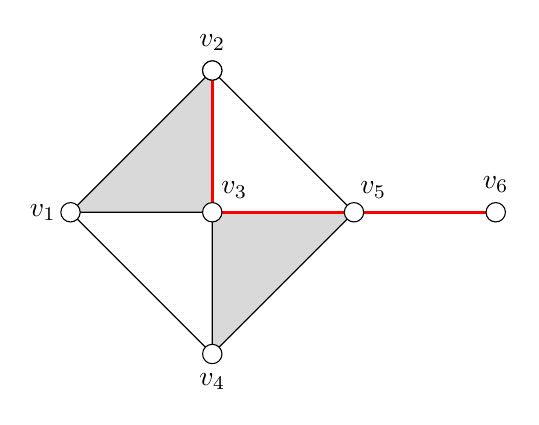
\begin{tikzpicture}[
            scale = .6,
            every node/.style={
              circle,
              draw=black,
              fill=white,
              inner sep=0pt,
              minimum size=7pt
            }
            ]

            \coordinate (v1) at (-3,0);
            \coordinate (v2) at (0,3);
            \coordinate (v3) at (0,0);
            \coordinate (v4) at (0,-3);
            \coordinate (v5) at (3,0);
            \coordinate (v6) at (6,0);

            \draw[fill=gray!30!white] (v1) -- (v2) -- (v3) -- (v1) -- cycle;
            \draw[fill=gray!30!white] (v3) -- (v4) -- (v5) -- (v3) -- cycle;

            \draw (v1) -- (v4);
            \draw (v2) -- (v5);
            \draw (v5) -- (v6);

            \draw[draw=red, very thick] (v6) -- (v5) -- (v3) -- (v2);

            \node (wv1) at (v1) {};
            \node (wv2) at (v2) {};
            \node (vv2) at (v2) {};
            \node (vv3) at (v3) {};
            \node (vv4) at (v4) {};
            \node (vv5) at (v5) {};
            \node (vv6) at (v6) {};

            \node[draw=none, xshift=-1em] (wv1) at (v1) {$v_1$};
            \node[draw=none, yshift=1em] (wv2) at (v2) {$v_2$};
            \node[draw=none, xshift=.8em, yshift=.8em] (wv3) at (v3) {$v_3$};
            \node[draw=none, yshift=-1em] (wv4) at (v4) {$v_4$};
            \node[draw=none, xshift=.7em, yshift=.8em] (wv5) at (v5) {$v_5$};
            \node[draw=none, yshift=1em] (wv6) at (v6) {$v_6$};
          \end{tikzpicture}
        \end{subfigure}
        \begin{subfigure}{.49\linewidth}
          \centering
          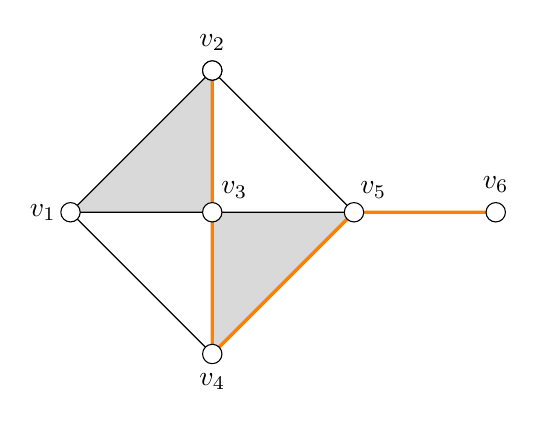
\begin{tikzpicture}[
            scale = .6,
            every node/.style={
              circle,
              draw=black,
              fill=white,
              inner sep=0pt,
              minimum size=7pt
            }
            ]

            \coordinate (v1) at (-3,0);
            \coordinate (v2) at (0,3);
            \coordinate (v3) at (0,0);
            \coordinate (v4) at (0,-3);
            \coordinate (v5) at (3,0);
            \coordinate (v6) at (6,0);

            \draw[fill=gray!30!white] (v1) -- (v2) -- (v3) -- (v1) -- cycle;
            \draw[fill=gray!30!white] (v3) -- (v4) -- (v5) -- (v3) -- cycle;

            \draw (v1) -- (v4);
            \draw (v2) -- (v5);
            \draw (v5) -- (v6);

            \draw[draw=orange, very thick] (v6) -- (v5) -- (v4) -- (v3)-- (v2);

            \node (wv1) at (v1) {};
            \node (wv2) at (v2) {};
            \node (vv2) at (v2) {};
            \node (vv3) at (v3) {};
            \node (vv4) at (v4) {};
            \node (vv5) at (v5) {};
            \node (vv6) at (v6) {};

            \node[draw=none, xshift=-1em] (wv1) at (v1) {$v_1$};
            \node[draw=none, yshift=1em] (wv2) at (v2) {$v_2$};
            \node[draw=none, xshift=.8em, yshift=.8em] (wv3) at (v3) {$v_3$};
            \node[draw=none, yshift=-1em] (wv4) at (v4) {$v_4$};
            \node[draw=none, xshift=.7em, yshift=.8em] (wv5) at (v5) {$v_5$};
            \node[draw=none, yshift=1em] (wv6) at (v6) {$v_6$};
          \end{tikzpicture}
        \end{subfigure}
        \begin{subfigure}{.49\linewidth}
          \centering
          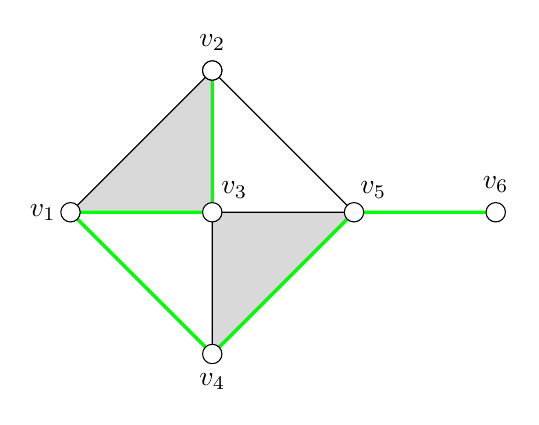
\begin{tikzpicture}[
            scale = .6,
            every node/.style={
              circle,
              draw=black,
              fill=white,
              inner sep=0pt,
              minimum size=7pt
            }
            ]

            \coordinate (v1) at (-3,0);
            \coordinate (v2) at (0,3);
            \coordinate (v3) at (0,0);
            \coordinate (v4) at (0,-3);
            \coordinate (v5) at (3,0);
            \coordinate (v6) at (6,0);

            \draw[fill=gray!30!white] (v1) -- (v2) -- (v3) -- (v1) -- cycle;
            \draw[fill=gray!30!white] (v3) -- (v4) -- (v5) -- (v3) -- cycle;

            \draw (v1) -- (v4);
            \draw (v2) -- (v5);
            \draw (v5) -- (v6);

            \draw[draw=green, very thick] (v6) -- (v5) -- (v4) -- (v1) -- (v3) -- (v2);

            \node (wv1) at (v1) {};
            \node (wv2) at (v2) {};
            \node (vv2) at (v2) {};
            \node (vv3) at (v3) {};
            \node (vv4) at (v4) {};
            \node (vv5) at (v5) {};
            \node (vv6) at (v6) {};

            \node[draw=none, xshift=-1em] (wv1) at (v1) {$v_1$};
            \node[draw=none, yshift=1em] (wv2) at (v2) {$v_2$};
            \node[draw=none, xshift=.8em, yshift=.8em] (wv3) at (v3) {$v_3$};
            \node[draw=none, yshift=-1em] (wv4) at (v4) {$v_4$};
            \node[draw=none, xshift=.7em, yshift=.8em] (wv5) at (v5) {$v_5$};
            \node[draw=none, yshift=1em] (wv6) at (v6) {$v_6$};
          \end{tikzpicture}
        \end{subfigure}
      \end{figure}\clearpage
      \begin{figure}[H]\ContinuedFloat
        \begin{subfigure}{.49\linewidth}
          \centering
          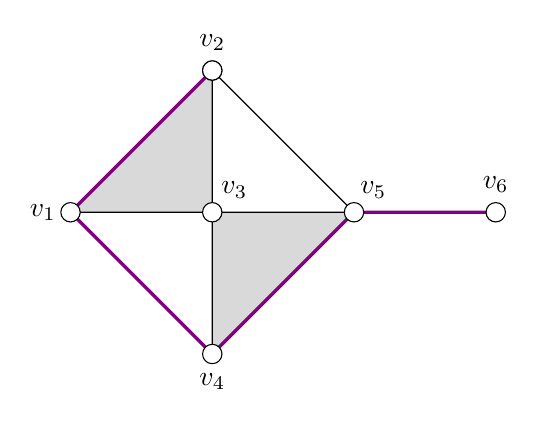
\begin{tikzpicture}[
            scale = .6,
            every node/.style={
              circle,
              draw=black,
              fill=white,
              inner sep=0pt,
              minimum size=7pt
            }
            ]

            \coordinate (v1) at (-3,0);
            \coordinate (v2) at (0,3);
            \coordinate (v3) at (0,0);
            \coordinate (v4) at (0,-3);
            \coordinate (v5) at (3,0);
            \coordinate (v6) at (6,0);

            \draw[fill=gray!30!white] (v1) -- (v2) -- (v3) -- (v1) -- cycle;
            \draw[fill=gray!30!white] (v3) -- (v4) -- (v5) -- (v3) -- cycle;

            \draw (v1) -- (v4);
            \draw (v2) -- (v5);
            \draw (v5) -- (v6);

            \draw[draw=violet, very thick] (v6) -- (v5) -- (v4) -- (v1)-- (v2);

            \node (wv1) at (v1) {};
            \node (wv2) at (v2) {};
            \node (vv2) at (v2) {};
            \node (vv3) at (v3) {};
            \node (vv4) at (v4) {};
            \node (vv5) at (v5) {};
            \node (vv6) at (v6) {};

            \node[draw=none, xshift=-1em] (wv1) at (v1) {$v_1$};
            \node[draw=none, yshift=1em] (wv2) at (v2) {$v_2$};
            \node[draw=none, xshift=.8em, yshift=.8em] (wv3) at (v3) {$v_3$};
            \node[draw=none, yshift=-1em] (wv4) at (v4) {$v_4$};
            \node[draw=none, xshift=.7em, yshift=.8em] (wv5) at (v5) {$v_5$};
            \node[draw=none, yshift=1em] (wv6) at (v6) {$v_6$};
          \end{tikzpicture}
        \end{subfigure}
        \begin{subfigure}{.49\linewidth}
          \centering
          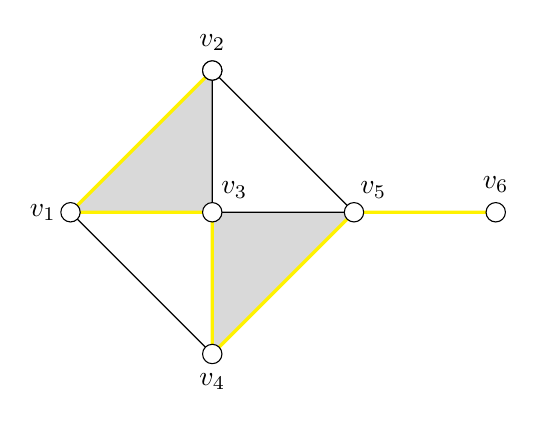
\begin{tikzpicture}[
            scale = .6,
            every node/.style={
              circle,
              draw=black,
              fill=white,
              inner sep=0pt,
              minimum size=7pt
            }
            ]

            \coordinate (v1) at (-3,0);
            \coordinate (v2) at (0,3);
            \coordinate (v3) at (0,0);
            \coordinate (v4) at (0,-3);
            \coordinate (v5) at (3,0);
            \coordinate (v6) at (6,0);

            \draw[fill=gray!30!white] (v1) -- (v2) -- (v3) -- (v1) -- cycle;
            \draw[fill=gray!30!white] (v3) -- (v4) -- (v5) -- (v3) -- cycle;

            \draw (v1) -- (v4);
            \draw (v2) -- (v5);
            \draw (v5) -- (v6);

            \draw[draw=yellow, very thick] (v6) -- (v5) -- (v4) -- (v3) -- (v1) -- (v2);

            \node (wv1) at (v1) {};
            \node (wv2) at (v2) {};
            \node (vv2) at (v2) {};
            \node (vv3) at (v3) {};
            \node (vv4) at (v4) {};
            \node (vv5) at (v5) {};
            \node (vv6) at (v6) {};

            \node[draw=none, xshift=-1em] (wv1) at (v1) {$v_1$};
            \node[draw=none, yshift=1em] (wv2) at (v2) {$v_2$};
            \node[draw=none, xshift=.8em, yshift=.8em] (wv3) at (v3) {$v_3$};
            \node[draw=none, yshift=-1em] (wv4) at (v4) {$v_4$};
            \node[draw=none, xshift=.7em, yshift=.8em] (wv5) at (v5) {$v_5$};
            \node[draw=none, yshift=1em] (wv6) at (v6) {$v_6$};
          \end{tikzpicture}
        \end{subfigure}
        \caption{Some paths from $v_6$ to $v_2$}
      \end{figure}
      among others. Taking the sum of the constituent edges in each path
      yields a sum of $1$-simplices with boundary $v_6,
      v_2$.\footnote{Justification: note that the coefficient on any given
        vertex when we apply $\partial$ is the degree of the vertex in our
        path. Hence, only the initial and terminal vertex don't get mapped
        to $0$.}
    \item Since $\msf B_n(K)$ is the group of all collections of even
      vertices in $\msf C_n(K)$, we have $\msf H_n(K) = \msf C_n(K)/\msf
      B_n(K) \cong \zmod{2}$.
    \end{enumerate}
  \item Now, we calculate the $k=1$ case.
    \begin{enumerate}
    \item Elements of $\msf C_1(K)$ are collections of linear combinations
      of the edges
      \[
        \msf C_1(K) = \ip{e_1, e_2, e_3, e_4, e_5, e_6, e_7, e_8, e_9}
      \]
    \item Elements of $\msf Z_1(K)$ are collections of edges such that
      each vertex contained in an edge in the collection has even degree.
      This corresponds to cyclic subgraphs of $K$ (as well as the empty
      cycle), e.g.:
      \begin{figure}[H]
        \centering
        \begin{subfigure}{.49\linewidth}
          \centering
          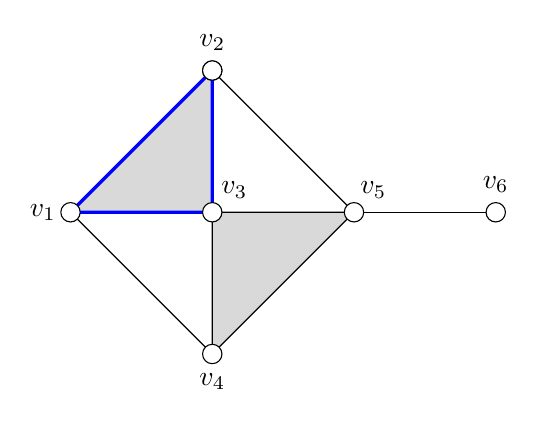
\begin{tikzpicture}[
            scale = .6,
            every node/.style={
              circle,
              draw=black,
              fill=white,
              inner sep=0pt,
              minimum size=7pt
            }
            ]

            \coordinate (v1) at (-3,0);
            \coordinate (v2) at (0,3);
            \coordinate (v3) at (0,0);
            \coordinate (v4) at (0,-3);
            \coordinate (v5) at (3,0);
            \coordinate (v6) at (6,0);

            \draw[fill=gray!30!white] (v1) -- (v2) -- (v3) -- (v1) -- cycle;
            \draw[fill=gray!30!white] (v3) -- (v4) -- (v5) -- (v3) -- cycle;

            \draw (v1) -- (v4);
            \draw (v2) -- (v5);
            \draw (v5) -- (v6);

            \draw[draw=blue, very thick] (v1) -- (v2) -- (v3) -- cycle;

            \node (wv1) at (v1) {};
            \node (wv2) at (v2) {};
            \node (vv2) at (v2) {};
            \node (vv3) at (v3) {};
            \node (vv4) at (v4) {};
            \node (vv5) at (v5) {};
            \node (vv6) at (v6) {};

            \node[draw=none, xshift=-1em] (wv1) at (v1) {$v_1$};
            \node[draw=none, yshift=1em] (wv2) at (v2) {$v_2$};
            \node[draw=none, xshift=.8em, yshift=.8em] (wv3) at (v3) {$v_3$};
            \node[draw=none, yshift=-1em] (wv4) at (v4) {$v_4$};
            \node[draw=none, xshift=.7em, yshift=.8em] (wv5) at (v5) {$v_5$};
            \node[draw=none, yshift=1em] (wv6) at (v6) {$v_6$};
          \end{tikzpicture}
        \end{subfigure}
        \begin{subfigure}{.49\linewidth}
          \centering
          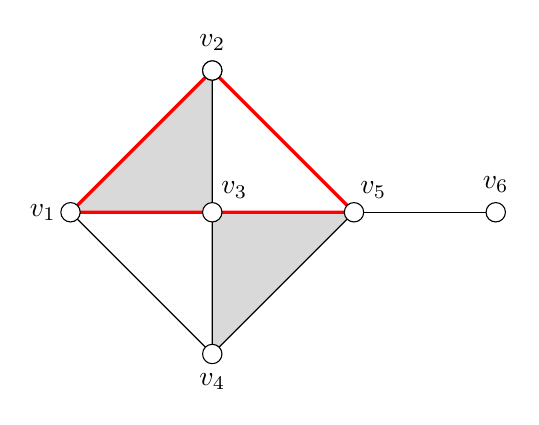
\begin{tikzpicture}[
            scale = .6,
            every node/.style={
              circle,
              draw=black,
              fill=white,
              inner sep=0pt,
              minimum size=7pt
            }
            ]

            \coordinate (v1) at (-3,0);
            \coordinate (v2) at (0,3);
            \coordinate (v3) at (0,0);
            \coordinate (v4) at (0,-3);
            \coordinate (v5) at (3,0);
            \coordinate (v6) at (6,0);

            \draw[fill=gray!30!white] (v1) -- (v2) -- (v3) -- (v1) -- cycle;
            \draw[fill=gray!30!white] (v3) -- (v4) -- (v5) -- (v3) -- cycle;

            \draw (v1) -- (v4);
            \draw (v2) -- (v5);
            \draw (v5) -- (v6);

            \draw[draw=red, very thick] (v1) -- (v2) -- (v5) -- (v3) -- (v1);

            \node (wv1) at (v1) {};
            \node (wv2) at (v2) {};
            \node (vv2) at (v2) {};
            \node (vv3) at (v3) {};
            \node (vv4) at (v4) {};
            \node (vv5) at (v5) {};
            \node (vv6) at (v6) {};

            \node[draw=none, xshift=-1em] (wv1) at (v1) {$v_1$};
            \node[draw=none, yshift=1em] (wv2) at (v2) {$v_2$};
            \node[draw=none, xshift=.8em, yshift=.8em] (wv3) at (v3) {$v_3$};
            \node[draw=none, yshift=-1em] (wv4) at (v4) {$v_4$};
            \node[draw=none, xshift=.7em, yshift=.8em] (wv5) at (v5) {$v_5$};
            \node[draw=none, yshift=1em] (wv6) at (v6) {$v_6$};
          \end{tikzpicture}
        \end{subfigure}
      \end{figure}
      \clearpage
      \begin{figure}[H]\ContinuedFloat
        \begin{subfigure}{.49\linewidth}
          \centering
          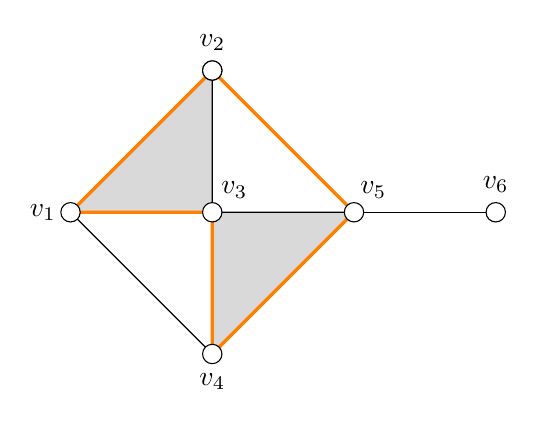
\begin{tikzpicture}[
            scale = .6,
            every node/.style={
              circle,
              draw=black,
              fill=white,
              inner sep=0pt,
              minimum size=7pt
            }
            ]

            \coordinate (v1) at (-3,0);
            \coordinate (v2) at (0,3);
            \coordinate (v3) at (0,0);
            \coordinate (v4) at (0,-3);
            \coordinate (v5) at (3,0);
            \coordinate (v6) at (6,0);

            \draw[fill=gray!30!white] (v1) -- (v2) -- (v3) -- (v1) -- cycle;
            \draw[fill=gray!30!white] (v3) -- (v4) -- (v5) -- (v3) -- cycle;

            \draw (v1) -- (v4);
            \draw (v2) -- (v5);
            \draw (v5) -- (v6);

            \draw[draw=orange, very thick] (v1) -- (v2) -- (v5) -- (v4)-- (v3) -- cycle;

            \node (wv1) at (v1) {};
            \node (wv2) at (v2) {};
            \node (vv2) at (v2) {};
            \node (vv3) at (v3) {};
            \node (vv4) at (v4) {};
            \node (vv5) at (v5) {};
            \node (vv6) at (v6) {};

            \node[draw=none, xshift=-1em] (wv1) at (v1) {$v_1$};
            \node[draw=none, yshift=1em] (wv2) at (v2) {$v_2$};
            \node[draw=none, xshift=.8em, yshift=.8em] (wv3) at (v3) {$v_3$};
            \node[draw=none, yshift=-1em] (wv4) at (v4) {$v_4$};
            \node[draw=none, xshift=.7em, yshift=.8em] (wv5) at (v5) {$v_5$};
            \node[draw=none, yshift=1em] (wv6) at (v6) {$v_6$};
          \end{tikzpicture}
        \end{subfigure}
        \begin{subfigure}{.49\linewidth}
          \centering
          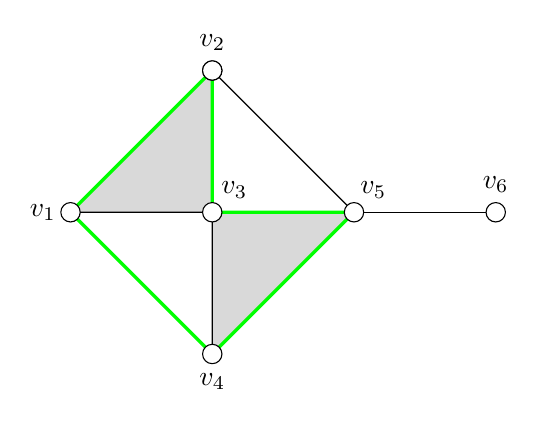
\begin{tikzpicture}[
            scale = .6,
            every node/.style={
              circle,
              draw=black,
              fill=white,
              inner sep=0pt,
              minimum size=7pt
            }
            ]

            \coordinate (v1) at (-3,0);
            \coordinate (v2) at (0,3);
            \coordinate (v3) at (0,0);
            \coordinate (v4) at (0,-3);
            \coordinate (v5) at (3,0);
            \coordinate (v6) at (6,0);

            \draw[fill=gray!30!white] (v1) -- (v2) -- (v3) -- (v1) -- cycle;
            \draw[fill=gray!30!white] (v3) -- (v4) -- (v5) -- (v3) -- cycle;

            \draw (v1) -- (v4);
            \draw (v2) -- (v5);
            \draw (v5) -- (v6);

            \draw[draw=green, very thick] (v1) -- (v2) -- (v3) -- (v5) -- (v4) -- cycle;

            \node (wv1) at (v1) {};
            \node (wv2) at (v2) {};
            \node (vv2) at (v2) {};
            \node (vv3) at (v3) {};
            \node (vv4) at (v4) {};
            \node (vv5) at (v5) {};
            \node (vv6) at (v6) {};

            \node[draw=none, xshift=-1em] (wv1) at (v1) {$v_1$};
            \node[draw=none, yshift=1em] (wv2) at (v2) {$v_2$};
            \node[draw=none, xshift=.8em, yshift=.8em] (wv3) at (v3) {$v_3$};
            \node[draw=none, yshift=-1em] (wv4) at (v4) {$v_4$};
            \node[draw=none, xshift=.7em, yshift=.8em] (wv5) at (v5) {$v_5$};
            \node[draw=none, yshift=1em] (wv6) at (v6) {$v_6$};
          \end{tikzpicture}
        \end{subfigure}
        \begin{subfigure}{.49\linewidth}
          \centering
          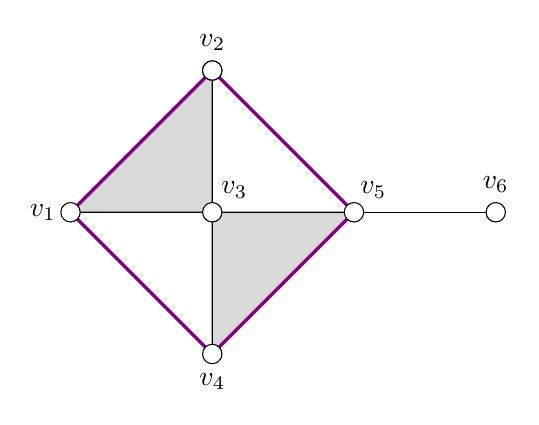
\begin{tikzpicture}[
            scale = .6,
            every node/.style={
              circle,
              draw=black,
              fill=white,
              inner sep=0pt,
              minimum size=7pt
            }
            ]

            \coordinate (v1) at (-3,0);
            \coordinate (v2) at (0,3);
            \coordinate (v3) at (0,0);
            \coordinate (v4) at (0,-3);
            \coordinate (v5) at (3,0);
            \coordinate (v6) at (6,0);

            \draw[fill=gray!30!white] (v1) -- (v2) -- (v3) -- (v1) -- cycle;
            \draw[fill=gray!30!white] (v3) -- (v4) -- (v5) -- (v3) -- cycle;

            \draw (v1) -- (v4);
            \draw (v2) -- (v5);
            \draw (v5) -- (v6);

            \draw[draw=violet, very thick] (v1) -- (v2) -- (v5) -- (v4) -- cycle;

            \node (wv1) at (v1) {};
            \node (wv2) at (v2) {};
            \node (vv2) at (v2) {};
            \node (vv3) at (v3) {};
            \node (vv4) at (v4) {};
            \node (vv5) at (v5) {};
            \node (vv6) at (v6) {};

            \node[draw=none, xshift=-1em] (wv1) at (v1) {$v_1$};
            \node[draw=none, yshift=1em] (wv2) at (v2) {$v_2$};
            \node[draw=none, xshift=.8em, yshift=.8em] (wv3) at (v3) {$v_3$};
            \node[draw=none, yshift=-1em] (wv4) at (v4) {$v_4$};
            \node[draw=none, xshift=.7em, yshift=.8em] (wv5) at (v5) {$v_5$};
            \node[draw=none, yshift=1em] (wv6) at (v6) {$v_6$};
          \end{tikzpicture}
        \end{subfigure}
        \begin{subfigure}{.49\linewidth}
          \centering
          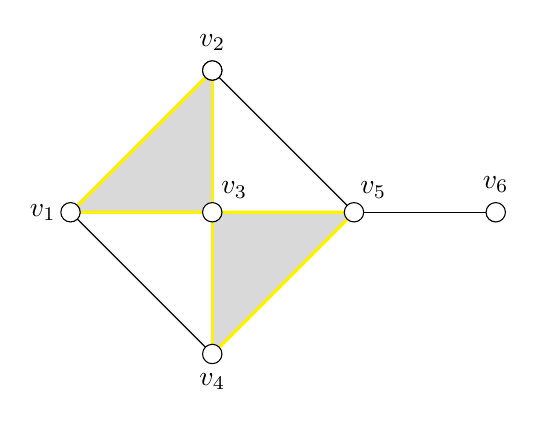
\begin{tikzpicture}[
            scale = .6,
            every node/.style={
              circle,
              draw=black,
              fill=white,
              inner sep=0pt,
              minimum size=7pt
            }
            ]

            \coordinate (v1) at (-3,0);
            \coordinate (v2) at (0,3);
            \coordinate (v3) at (0,0);
            \coordinate (v4) at (0,-3);
            \coordinate (v5) at (3,0);
            \coordinate (v6) at (6,0);

            \draw[fill=gray!30!white] (v1) -- (v2) -- (v3) -- (v1) -- cycle;
            \draw[fill=gray!30!white] (v3) -- (v4) -- (v5) -- (v3) -- cycle;

            \draw (v1) -- (v4);
            \draw (v2) -- (v5);
            \draw (v5) -- (v6);

            \draw[draw=yellow, very thick] (v1) -- (v2) -- (v3) -- cycle;
            \draw[draw=yellow, very thick] (v3) -- (v4) -- (v5) -- cycle;

            \node (wv1) at (v1) {};
            \node (wv2) at (v2) {};
            \node (vv2) at (v2) {};
            \node (vv3) at (v3) {};
            \node (vv4) at (v4) {};
            \node (vv5) at (v5) {};
            \node (vv6) at (v6) {};

            \node[draw=none, xshift=-1em] (wv1) at (v1) {$v_1$};
            \node[draw=none, yshift=1em] (wv2) at (v2) {$v_2$};
            \node[draw=none, xshift=.8em, yshift=.8em] (wv3) at (v3) {$v_3$};
            \node[draw=none, yshift=-1em] (wv4) at (v4) {$v_4$};
            \node[draw=none, xshift=.7em, yshift=.8em] (wv5) at (v5) {$v_5$};
            \node[draw=none, yshift=1em] (wv6) at (v6) {$v_6$};
          \end{tikzpicture}
        \end{subfigure}
        \caption{Some cycles in $K$}
      \end{figure}
    \item First, consider the following diagram:
      \begin{figure}[H]
        \centering
        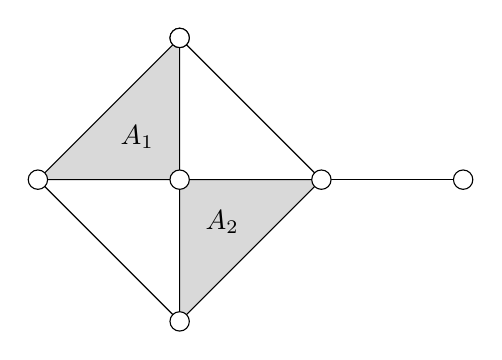
\begin{tikzpicture}[
          scale = .6,
          every node/.style={
            circle,
            draw=black,
            fill=white,
            inner sep=0pt,
            minimum size=7pt
          }
          ]

          \coordinate (v1) at (-3,0);
          \coordinate (v2) at (0,3);
          \coordinate (v3) at (0,0);
          \coordinate (v4) at (0,-3);
          \coordinate (v5) at (3,0);
          \coordinate (v6) at (6,0);

          \draw[fill=gray!30!white] (v1) -- (v2) -- (v3) -- (v1) -- cycle;

          \draw (v1) -- (v4);

          \draw[fill=gray!30!white] (v3) -- (v4) -- (v5) -- (v3) -- cycle;


          \draw (v2) -- (v5) ;
          \draw (v5) -- (v6) ;

          \node (wv1) at (v1) {};
          \node (wv2) at (v2) {};
          \node (vv2) at (v2) {};
          \node (vv3) at (v3) {};
          \node (vv4) at (v4) {};
          \node (vv5) at (v5) {};
          \node (vv6) at (v6) {};

          \node[draw=none,fill=none] (a1) at (-.9,.9) {$A_1$};
          \node[draw=none,fill=none] (a1) at (.9,-.9) {$A_2$};
        \end{tikzpicture}
        \caption{Two $n=2$ simplices}
      \end{figure}
      $\mb 0_1$ bounds $\mb 0_2$. Since $\partial(A_1) \cap \partial(A_2) =
      \varnothing$, then the other two cycles in $\msf B_1(K)$ are just
      $\partial(A_1)$ and $\partial(A_2)$, respectively.
    \item $\msf H_1(K) \cong \zmod{2} \times \zmod{2}$ (equivalence classes
      have representative elements $\mb 0, \partial(A_1), \partial(A_2),
      \partial(A_1) + \partial(A_2)$)
    \end{enumerate}
  \item For $k=2$, we have
    \begin{enumerate}
    \item $\msf C_2(K) \cong \zmod{2} \times \zmod{2}$
    \item $\msf Z_2(K) \cong \mb 0$
    \item $\msf B_2(K) \cong \mb 0$
    \item And hence $\msf H_2(K) \cong \mb 0$.
    \end{enumerate}
  \end{enumerate}
\end{solution}
\begin{problem}[16.7]
  If $K$ is a one-point space, $\msf H_n(K) \cong 0$ for $n \geq 0$, and $\msf
  H_0(K) \cong \zmod{2}$.
\end{problem}
\begin{solution}
  For $n > 0$, $\msf C_n(K)$ is the trivial group. Since $\msf Z_n(K) \leq \msf
  C_n(K)$, we thus have $\msf Z_n(K) \cong 0$, and so $\msf H_n(K) \cong 0$.

  For the $n = 0$, note that $\msf Z_0(K) = \msf C_0(K) \cong \zmod{2}$ (every
  point is definitionally a 0-cycle). Since $K$ contains no 1-simplices, $\msf
  B_0(K) = \mb 0$, hence $\msf H_0(K) \cong \zmod{2}$.
\end{solution}
\begin{definition}[Simplicially connected]
  Let $K$ be a simplicial complex. Then we call $K$ \emph{simplicially
    connected} iff for all pairs of 0-simplices $v_0, v_n \in K$, there exists a
  sequence of 0-simplices $\set{v_i}_{i\in [n]}$ such that for all $i \in [n]$
  (with $i \neq n$), $\set{v_iv_{i+1}}$ is a 1-simplex in $K$. Note, this
  corresponds exactly to $K$ being connected as a graph, where the 0-simplices
  represent vertices, and the 1-simplices represent edges.
\end{definition}
\begin{problem}[16.8]
  If $K$ is simplicially connected, then $\msf H_0(K) \cong \zmod{2}$. If $K$
  has $r$ simplicially connected components, then
  \[
    \msf H_0(K)\cong \prod_{i=1}^r \zmod{2}
  \]
\end{problem}
\begin{solution}
  \begin{enumerate}
  \item Suppose $K$ is simplicially connected. We want to show $\msf H_0(K)
    \cong \zmod{2}$. First, observe that $\msf Z_0(K) \cong \msf C_0(K)$
    (every 0 simplex has trivial boundary). By properties of module
    homomorphisms, for all $\sigma \in \msf B_0(K)$, $\sigma$ is a basis
    element of $\msf B_0(K)$ iff $\exists \tau \in \msf C_1(K)$ such that
    $\tau$ is a basis element of $\msf C_1(K)$, and $\partial_1(\tau) =
    \sigma$. Thus, $\msf B_0(K)$ is spanned by $\set{\set{\set{v_i} +
        \set{v_j}} \MID \set{v_iv_j} \in K}$. It follows that $\msf B_0(K)$
    contains exactly those elements of $\msf C_0(K)$ with an even number of
    vertices.\footnote{Since $\msf B_0(K)$ is generated by pairs.}

    It follows that $\msf H_0(K) = \msf Z_0(K)/\msf B_0(K) \cong \zmod{2}$
    (any $0$-chain has either an even or odd number of vertices).
  \item This follows by applying the above argument to each of the connected
    components.
  \end{enumerate}
\end{solution}
\begin{problem}[16.9]
  Let $K$ be a triangulation of a $3$-dimensional ball that consists of a
  3-simplex together with its faces. Compute $\msf H_n(K)$ for each $n$.
\end{problem}
\begin{solution}
  \begin{figure}[H]
    \centering
    \begin{subfigure}{\linewidth}
      \centering
      \tdplotsetmaincoords{70}{80}
      \begin{tikzpicture}[tdplot_main_coords,scale=2]
        \path
        coordinate (A) at (0,0,0)
        coordinate (B) at (2,0,0)
        coordinate (C) at (1,1.732,0)
        coordinate (D) at (1,.577,1.733);

        \draw [dashed] (A)--(C);
        \fill [opacity=.5, red!30!white] (A) -- (B) -- (C) -- cycle;
        \fill [opacity=.5, blue!30!white] (D) -- (B) -- (A) -- cycle;
        \fill [opacity=.5, green!30!white] (D) -- (A) -- (C) -- cycle;
        \draw[thick] (A) -- (B) (A) -- (D);
        \draw[thick, fill opacity=.5, fill=orange!30!white] (D) -- (B) -- (C) -- cycle;

        \node (V) at (1,.577,.433) {\LARGE $V_1$};

        \foreach \v/\position in {A/left,B/below,C/right,D/above} {
          \draw[fill=black] (\v) circle (0.5pt) node [\position=0.2mm] {$\v$};
        }
      \end{tikzpicture}
    \end{subfigure}\\\vspace{1cm}
    \begin{subfigure}{.24\linewidth}
      \centering
      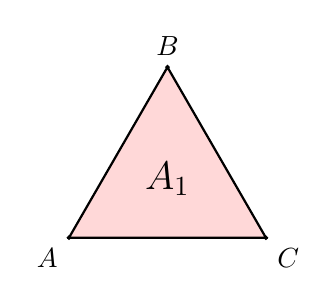
\begin{tikzpicture}[scale=1.25]
        \path
        coordinate (A) at (0,0)
        coordinate (C) at (2,0)
        coordinate (B) at (1,1.732);

        \draw[thick, fill opacity=.5, fill=red!30!white] (A) -- (B) -- (C) -- cycle;

        \node (A1) at (1,.6) {\Large $A_1$};

        \foreach \v/\position in {A/below left, C/below right, B/above} {
          \draw[fill=black] (\v) circle (0.5pt) node [\position=0.2mm] {$\v$};
        }
      \end{tikzpicture}
    \end{subfigure}
    \begin{subfigure}{.24\linewidth}
      \centering
      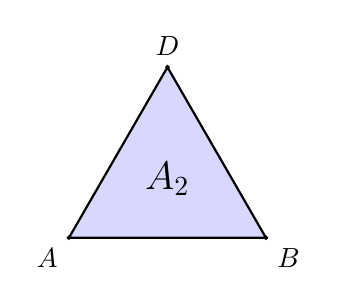
\begin{tikzpicture}[scale=1.25]
        \path
        coordinate (A) at (0,0)
        coordinate (B) at (2,0)
        coordinate (D) at (1,1.732);

        \draw[thick, fill opacity=.5, fill=blue!30!white] (D) -- (B) -- (A) -- cycle;

        \node (A2) at (1,.6) {\Large $A_2$};

        \foreach \v/\position in {A/below left, B/below right, D/above} {
          \draw[fill=black] (\v) circle (0.5pt) node [\position=0.2mm] {$\v$};
        }
      \end{tikzpicture}
    \end{subfigure}
    \begin{subfigure}{.24\linewidth}
      \centering
      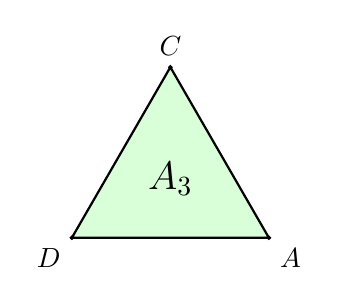
\begin{tikzpicture}[scale=1.25]
        \path
        coordinate (D) at (0,0)
        coordinate (A) at (2,0)
        coordinate (C) at (1,1.732);

        \draw[thick, fill opacity=.5, fill=green!30!white] (D) -- (A) -- (C) -- cycle;

        \node (A3) at (1,.6) {\Large $A_3$};

        \foreach \v/\position in {D/below left, A/below right, C/above} {
          \draw[fill=black] (\v) circle (0.5pt) node [\position=0.2mm] {$\v$};
        }
      \end{tikzpicture}
    \end{subfigure}
    \begin{subfigure}{.24\linewidth}
      \centering
      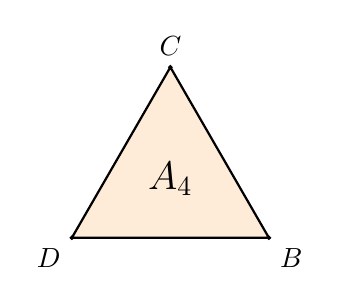
\begin{tikzpicture}[scale=1.25]
        \path
        coordinate (D) at (0,0)
        coordinate (B) at (2,0)
        coordinate (C) at (1,1.732);

        \draw[thick, fill opacity=.5, fill=orange!30!white] (D) -- (B) -- (C) -- cycle;

        \node (A4) at (1,.6) {\Large $A_4$};

        \foreach \v/\position in {D/below left, B/below right, C/above} {
          \draw[fill=black] (\v) circle (0.5pt) node [\position=0.2mm] {$\v$};
        }
      \end{tikzpicture}
    \end{subfigure}\\\vspace{1cm}
    \tikzset{
      brace/.style={
        thick,
        decoration={brace, mirror, raise=1pt, amplitude=6pt},
        decorate
      },
      blabel/.style={
        right, pos=.5, xshift=7pt, yshift=-2pt
      }
    }
    \begin{subfigure}{.161\linewidth}
      \centering
      \begin{tikzpicture}[scale=1.25]
        \def\firstcoord{A}
        \def\secondcoord{B}
        \path coordinate (\firstcoord) at (0,0) coordinate (\secondcoord) at (0,1.73);
        \draw[thick] (\firstcoord) -- (\secondcoord);

        \draw[brace] (.3,-.4) -- node[blabel] {\Large $e_1$} (.3,2.13);

        \foreach \v/\position in {\firstcoord/below, \secondcoord/above} {
          \draw[fill=black] (\v) circle (0.5pt) node [\position=0.2mm] {$\v$};
        }
      \end{tikzpicture}
    \end{subfigure}
    \begin{subfigure}{.161\linewidth}
      \centering
      \begin{tikzpicture}[scale=1.25]
        \def\firstcoord{A}
        \def\secondcoord{C}
        \path coordinate (\firstcoord) at (0,0) coordinate (\secondcoord) at (0,1.73);
        \draw[thick] (\firstcoord) -- (\secondcoord);

        \draw[brace] (.3,-.4) -- node[blabel] {\Large $e_2$} (.3,2.13);

        \foreach \v/\position in {\firstcoord/below, \secondcoord/above} {
          \draw[fill=black] (\v) circle (0.5pt) node [\position=0.2mm] {$\v$};
        }
      \end{tikzpicture}
    \end{subfigure}
    \begin{subfigure}{.161\linewidth}
      \centering
      \begin{tikzpicture}[scale=1.25]
        \def\firstcoord{A}
        \def\secondcoord{D}
        \path coordinate (\firstcoord) at (0,0) coordinate (\secondcoord) at (0,1.73);
        \draw[thick] (\firstcoord) -- (\secondcoord);

        \draw[brace] (.3,-.4) -- node[blabel] {\Large $e_3$} (.3,2.13);

        \foreach \v/\position in {\firstcoord/below, \secondcoord/above} {
          \draw[fill=black] (\v) circle (0.5pt) node [\position=0.2mm] {$\v$};
        }
      \end{tikzpicture}
    \end{subfigure}
    \begin{subfigure}{.161\linewidth}
      \centering
      \begin{tikzpicture}[scale=1.25]
        \def\firstcoord{B}
        \def\secondcoord{C}
        \path coordinate (\firstcoord) at (0,0) coordinate (\secondcoord) at (0,1.73);
        \draw[thick] (\firstcoord) -- (\secondcoord);

        \draw[brace] (.3,-.4) -- node[blabel] {\Large $e_4$} (.3,2.13);

        \foreach \v/\position in {\firstcoord/below, \secondcoord/above} {
          \draw[fill=black] (\v) circle (0.5pt) node [\position=0.2mm] {$\v$};
        }
      \end{tikzpicture}
    \end{subfigure}
    \begin{subfigure}{.161\linewidth}
      \centering
      \begin{tikzpicture}[scale=1.25]
        \def\firstcoord{B}
        \def\secondcoord{D}
        \path coordinate (\firstcoord) at (0,0) coordinate (\secondcoord) at (0,1.73);
        \draw[thick] (\firstcoord) -- (\secondcoord);

        \draw[brace] (.3,-.4) -- node[blabel] {\Large $e_5$} (.3,2.13);

        \foreach \v/\position in {\firstcoord/below, \secondcoord/above} {
          \draw[fill=black] (\v) circle (0.5pt) node [\position=0.2mm] {$\v$};
        }
      \end{tikzpicture}
    \end{subfigure}
    \begin{subfigure}{.161\linewidth}
      \centering
      \begin{tikzpicture}[scale=1.25]
        \def\firstcoord{C}
        \def\secondcoord{D}
        \path coordinate (\firstcoord) at (0,0) coordinate (\secondcoord) at (0,1.73);
        \draw[thick] (\firstcoord) -- (\secondcoord);

        \draw[brace] (.3,-.4) -- node[blabel] {\Large $e_6$} (.3,2.13);

        \foreach \v/\position in {\firstcoord/below, \secondcoord/above} {
          \draw[fill=black] (\v) circle (0.5pt) node [\position=0.2mm] {$\v$};
        }
      \end{tikzpicture}
    \end{subfigure}\\\vspace{1.5cm}
    \begin{subfigure}{\linewidth}
      \centering
      \begin{tikzpicture}[scale=1.25]
        \path
        coordinate (A) at (-4,0)
        coordinate (B) at (-1.33,0)
        coordinate (C) at (1.33,0)
        coordinate (D) at (4,0);

        \foreach \v in {A,B,C,D} {
          \draw[fill=black] (\v) circle (2pt) node [below, yshift=-5pt] {$\v$};
        }
      \end{tikzpicture}
    \end{subfigure}\\\vspace{0cm}
    \caption{3-simplex and its basis faces. Note the 1, 4, 6, 4 relationship.
      Gotta love Pascal's 2-simplex!}
    \label{fig:circumscribed}
  \end{figure}
  \begin{enumerate}[label=(\arabic*)]\setcounter{enumi}{-1}
  \item $K$ is connected, so $\msf H_0(K) \cong \mb \zmod{2}$.
  \item Elements of $\msf B_1(K)$ are linear combinations of $\bdy[2]{A_1}$,
    $\bdy[2]{A_2}$, $\bdy[2]{A_3}$, and $\bdy[2]{A_4}$.
    \begin{itemize}
    \item Given any single edge, adding $A_i$
    \end{itemize}
  \item $\msf Z_2(K) = \set{\mb 0, A_1 + A_2 + A_3 + A_4} = B_2(K) \cong
    \zmod{2}$, so $\msf H_2(K) \cong \mb 0$.
  \item $\msf H_3(K) \cong \mb 0$.
  \end{enumerate}
\end{solution}
\begin{problem}[16.10]
  Let $K$ be a triangulation of a 2-sphere that consists of the proper faces of
  a 3-simplex. Compute $\msf H_n(K)$ for each $n$.
\end{problem}
\begin{solution}
  Proceed as before for $k=0,1$. For $k=2$, note $\msf B_2(K) \cong \mb 0$.
  Hence, $\msf H_2(K) \cong \zmod{2}$.
\end{solution}
\begin{definition}
  Let $K$ be a simplicial complex with $\abs{K} \subset \RR^n$. A point $x
  \not\in K$ can \emph{see} $K$ if any ray from $x$ intersects $\abs{K}$ at most
  once (as seen in the following diagram).
\end{definition}
\begin{figure}[H]
  \centering
  \begin{subfigure}{.49\linewidth}
    \centering
    \tdplotsetmaincoords{70}{80}
    \begin{tikzpicture}[tdplot_main_coords, scale=2]
      \path
      coordinate (B) at (2,0,0)
      coordinate (C) at (1,1.732,0)
      coordinate (x) at (.6,.577,1.533)
      coordinate (y) at (1.8,1.077,1.733);

      \draw (B)--(C);

      \path
      coordinate (P1) at ($.5*(B) + .5*(C)$)
      coordinate (P2) at ($.23*(B) + .77*(C)$)
      coordinate (P3) at ($.7*(B) + .3*(C)$)
      coordinate (P4) at ($.4*(B) + .6*(C)$);

      \foreach \v in {P1,P2,P3,P4}{
        % Take the difference and go slightly past it
        \draw[-latex,dashed,color=red!30!white] (x) -- ($1.3*(\v) - .3*(x)$);
        \draw[-latex,dashed,color=blue!30!white] (y) -- ($1.3*(\v) - .3*(y)$);
        \draw[fill=black] (\v) circle (0.5pt);
      }

      \foreach \v in {B,C}{
        % Take the difference and go slightly past it
        \draw[-latex,dashed,color=red!30!white] (x) -- ($1.2*(\v) - .2*(x)$);
        \draw[-latex,dashed,color=blue!30!white] (y) -- ($1.2*(\v) - .2*(y)$);
        \draw[fill=black] (\v) circle (0.5pt);
      }

      \foreach \v/\position in {B/left,C/right,x/above,y/above right} {
        \draw[fill=black] (\v) circle (0.5pt) node [\position=0.2mm] {$\v$};
      }
    \end{tikzpicture}
    \caption{$x$ and $y$ both see a $1$-simplex $\sigma_1$}
    \label{fig:see-sigma-1}
  \end{subfigure}
  \begin{subfigure}{.49\linewidth}
    \centering
    \tdplotsetmaincoords{70}{80}
    \begin{tikzpicture}[tdplot_main_coords, scale=2]
      \path
      coordinate (A) at (0,0,0)
      coordinate (B) at (2,0,0)
      coordinate (C) at (1,1.732,0)
      coordinate (x) at (1,.577,1.733);

      \fill[red!30!white,draw=black] (A)--(B)--(C)--cycle;

      \path
      coordinate (P1) at ($.2*(A) + .5*(B) + .4*(C)$)
      coordinate (P2) at ($.3*(A) + .5*(B) + .2*(C)$)
      coordinate (P3) at ($.2*(A) + .2*(B) + .6*(C)$)
      coordinate (P4) at ($.7*(A) + .2*(B) + .1*(C)$);

      \foreach \v in {P1,P2,P3,P4}{
        % Take the difference and go slightly past it
        \draw[-latex,dashed] (x) -- ($1.3*(\v) - .3*(x)$);
        \draw[fill=black] (\v) circle (0.5pt);
      }

      \foreach \v in {A,B,C}{
        % Take the difference and go slightly past it
        \draw[-latex,dashed] (x) -- ($1.2*(\v) - .2*(x)$);
        \draw[fill=black] (\v) circle (0.5pt);
      }

      \foreach \v/\position in {A/left,B/left,C/right,x/above} {
        \draw[fill=black] (\v) circle (0.5pt) node [\position=0.2mm] {$\v$};
      }
    \end{tikzpicture}
    \caption{$x$ sees a $2$-simplex $\sigma_2$}
    \label{fig:see-sigma-2}
  \end{subfigure}
  \caption{Simplices being seen}
  \label{fig:seeing}
\end{figure}
\begin{remark}
  Note, that when there are multiple $k$-simplices in $K$, the picture might not
  be quite as simple.
\end{remark}
\begin{definition}
  Let $K$ be a finite complex and $x$ a point that sees $K$. If $\sigma =
  \simp{k}$ is a simplex of $K$, define the \emph{cone} of $x$ over $\sigma$ to
  be the simplex
  \[
    \Cone_x(\sigma) = \set{xv_0\cdots v_k}.
  \]
\end{definition}
\begin{figure}[H]
  \centering
  \begin{subfigure}{.49\linewidth}
    \centering
    \tdplotsetmaincoords{70}{80}
    \begin{tikzpicture}[tdplot_main_coords, scale=2]
      \path
      coordinate (B) at (2,0,0)
      coordinate (C) at (1,1.732,0)
      coordinate (x) at (.6,.577,1.533)
      coordinate (y) at (1.8,1.077,1.733);

      \draw (B)--(C);

      \fill [opacity=.5, red!30!white] (x) -- (B) -- (C) -- cycle;
      \fill [opacity=.5, blue!30!white] (y) -- (B) -- (C) -- cycle;

      \draw[dashed] (x) -- (B) (x) -- (C);
      \draw[dashed] (y) -- (B) (y) -- (C);

      \foreach \v/\position in {B/left,C/right,x/above,y/above right} {
        \draw[fill=black] (\v) circle (0.5pt) node [\position=0.2mm] {$\v$};
      }
    \end{tikzpicture}
    \caption{$\Cone_x(\sigma_1)$, $\Cone_y(\sigma_1)$}
    \label{fig:cone-sigma-1}
  \end{subfigure}
  \begin{subfigure}{.49\linewidth}
    \centering
    \tdplotsetmaincoords{70}{80}
    \begin{tikzpicture}[tdplot_main_coords, scale=2]
      \path
      coordinate (A) at (0,0,0)
      coordinate (B) at (2,0,0)
      coordinate (C) at (1,1.732,0)
      coordinate (D) at (1,.577,1.733);

      \fill[red!30!white,draw=black] (A)--(B)--(C)--cycle;

      % Draw this first so it gets covered by the fill slightly
      \draw (A) -- (C);

      \fill [opacity=.5, red!30!white] (A) -- (B) -- (C) -- cycle;
      \fill [opacity=.5, blue!30!white] (D) -- (B) -- (A) -- cycle;
      \fill [opacity=.5, green!30!white] (D) -- (A) -- (C) -- cycle;
      \fill [opacity=.5, orange!30!white] (D) -- (B) -- (C) -- cycle;
      \draw[dashed] (A) -- (D) (B) -- (D) (C) -- (D);

      % Draw this first so it gets covered by the fill slightly
      \draw (A) -- (B) -- (C);

      \foreach \v/\position in {A/left,B/left,C/right,D/above} {
        \draw[fill=black] (\v) circle (0.5pt) node [\position=0.2mm] {$\v$};
      }
    \end{tikzpicture}
    \caption{$\Cone_x(\sigma_2)$}
    \label{fig:cone-sigma-2}
  \end{subfigure}
  \caption{Some cones}
  \label{fig:cones}
\end{figure}
\begin{definition}
  Define $x*K$, the \emph{cone over} $K$ to be the simplicial complex comprising
  all simplices $\Cone_x(\sigma)$ for $\sigma \in K$, and all faces of such
  simplices.
\end{definition}
\begin{remark}
  Essentially, this just includes the base point and edges in
  \cref{fig:cone-sigma-1} and the base point and edges \emph{and} faces in
  \cref{fig:cone-sigma-2}.
\end{remark}
\begin{definition}
  Define the \emph{simplicial cone operator} $\Cone_x : \msf C_n(K) \to \msf
  C_{n+1}(x*K)$ by extending the definition of $\Cone_x(\sigma)$ linearly to
  chains.
\end{definition}
\begin{problem}[16.11]
  For $x$ seeing $K$, and $\sigma$ a simplex of $K$,
  \[
    \partial\ \Cone_x(\sigma) + \Cone_x(\partial \sigma) = \sigma.
  \]
\end{problem}
\begin{solution}

\end{solution}
%%% Local Variables:
%%% TeX-master: "main"
%%% End:

\end{document}
%%% Local Variables:
%%% TeX-master: t
%%% TeX-engine: default-shell-escape
%%% TeX-command-extra-option: -pdf
%%% End: